%% abtex2-modelo-include-comandos.tex, v-1.9.6 laurocesar
%% Copyright 2012-2016 by abnTeX2 group at http://www.abntex.net.br/ 
%%
%% This work may be distributed and/or modified under the
%% conditions of the LaTeX Project Public License, either version 1.3
%% of this license or (at your option) any later version.
%% The latest version of this license is in
%%   http://www.latex-project.org/lppl.txt
%% and version 1.3 or later is part of all distributions of LaTeX
%% version 2005/12/01 or later.
%%
%% This work has the LPPL maintenance status `maintained'.
%% 
%% The Current Maintainer of this work is the abnTeX2 team, led
%% by Lauro César Araujo. Further information are available on 
%% http://www.abntex.net.br/
%%
%% This work consists of the files abntex2-modelo-include-comandos.tex
%% and abntex2-modelo-img-marca.pdf
%%

% ---
% Este capítulo, utilizado por diferentes exemplos do abnTeX2, ilustra o uso de
% comandos do abnTeX2 e de LaTeX.
% ---

\chapter{Novos Alótropos de Carbono}
\label{chap:novos_alotropos}
\section{Spiro-Carbon}
\label{sec:spiro}

	Em um trabalho desenvolvido pelo nosso grupo anteriormente ao desenvolvimento desta dissertação, foi explorada a existência de uma nova família de alótropos de carbono, denominada \textit{n}-diamantinos, sendo relatada em artigo publicado em \citeyear{costa2018n} \cite{costa2018n}. Esta família descreve uma generalização do conceito de formação de novas estruturas de carbono através da inserção de \textit{n} derivados de acetileno entre os átomos de carbono. 
	
	Se considerarmos que um dos membros desta família, o 1-diamantino que também relatado na literatura como Y-Carbon \cite{jo2012carbon}, poderia sofrer um rearranjo entre as ligações triplas vicinais (com mostrado na \autoref{soliton}),o  resultado seria a formação de dois anéis de três membros perpendiculares compartilhando um átomo de carbono entre si, um motivo estrutural conhecido como \textit{spiro}. Esse motivo estrutural resultante estaria conectado por ligações químicas formando uma estrutura periódica.

	\begin{figure}[ht]
		\centering
		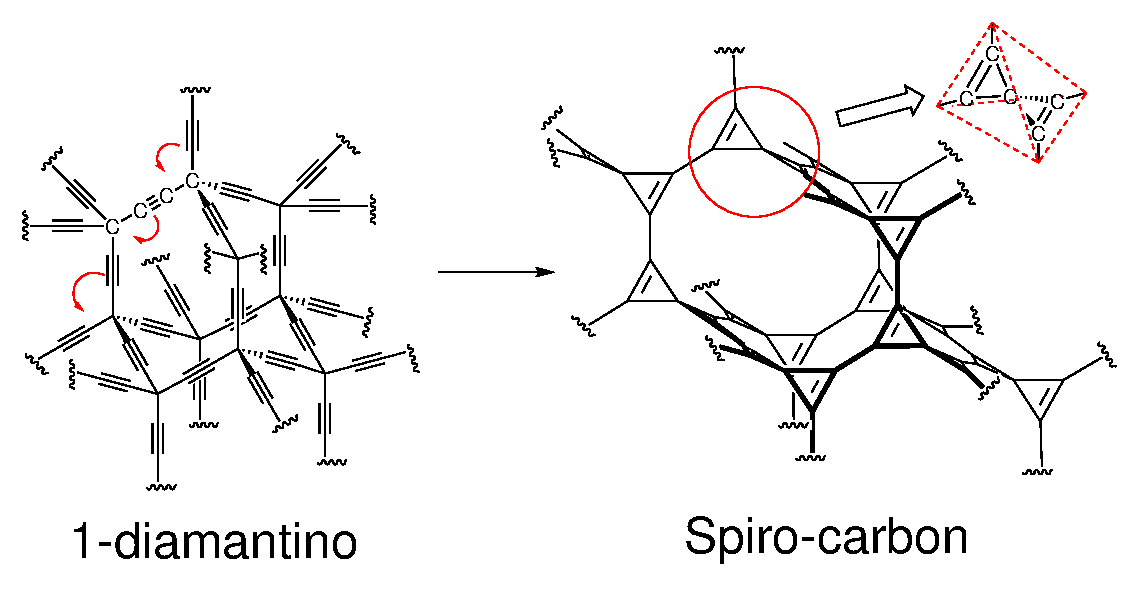
\includegraphics[width=1\linewidth]{capitulos/fig/results1/estrutura_1diamantino-spiro.eps}
		\caption{Rearranjo das cadeias geminais do 1-diamantino para formar um novo alótropo de carbono com o motivo estrutural \textit{spiro}.}
		\label{soliton}
	\end{figure}

	A síntese composto molecular que apresenta o motivo estrutural que forma esta estrutura, o spiropentadieno, já foi relatada na literatura em \citeyear{billups1991spiropentadiene} por \citeauthor{billups1991spiropentadiene}.\footnote{A estrutura desta molécula é apresentada em mais detalhes no Apêndice \autoref{chap:spiropentadiene}} Além disso, algumas variações estruturais dessa molécula já apresentaram propriedades interessantes. Ela já foi explorada, por exemplo, para propor um hidrocarboneto que poderia violar o paradigma químico de mais de 150 anos de que um átomo de carbono tetravalente e tetra-coordenado deve assumir um arranjo estrutural tetraédrico \cite{esteves2005neutral}. 
	
	No spiropentadieno neutro, dois anéis de três membros estão ortogonais entre sí, o que faz dessa molécula uma espécie tetraedro esticado. Dessa forma, poderíamos ligar esses tetraedros de uma maneira análoga à ligação dos átomos de carbono no diamante, gerando assim a estrutura de um novo alótropo de carbono.

	\subsection{Estrutura}

	A estrutura desse novo alótropo de carbono, denominada de Spiro-Carbon, contém 10 átomos em uma célula unitária primitiva tetragonal de corpo centrado, apresentando grupo espacial $I4_1/amd$ (\#141) e grupo pontual $D_{4h}$. A geometria resultante da otimização estrutural apresenta os parâmetros de célula \textit{a} = \textit{b} = 5.122 Å, \textit{c} = 13.126 Å e $\alpha$ = $\beta$ = $\gamma$ = 90$^\circ$, apresentando densidade de 1.16 g/cm$^3$. Representações da célula unitária vista por pelos diferentes vetores de célula são mostradas na \autoref{estrutura_spiro}
	
	\begin{figure}[hbt!]
		\centering
		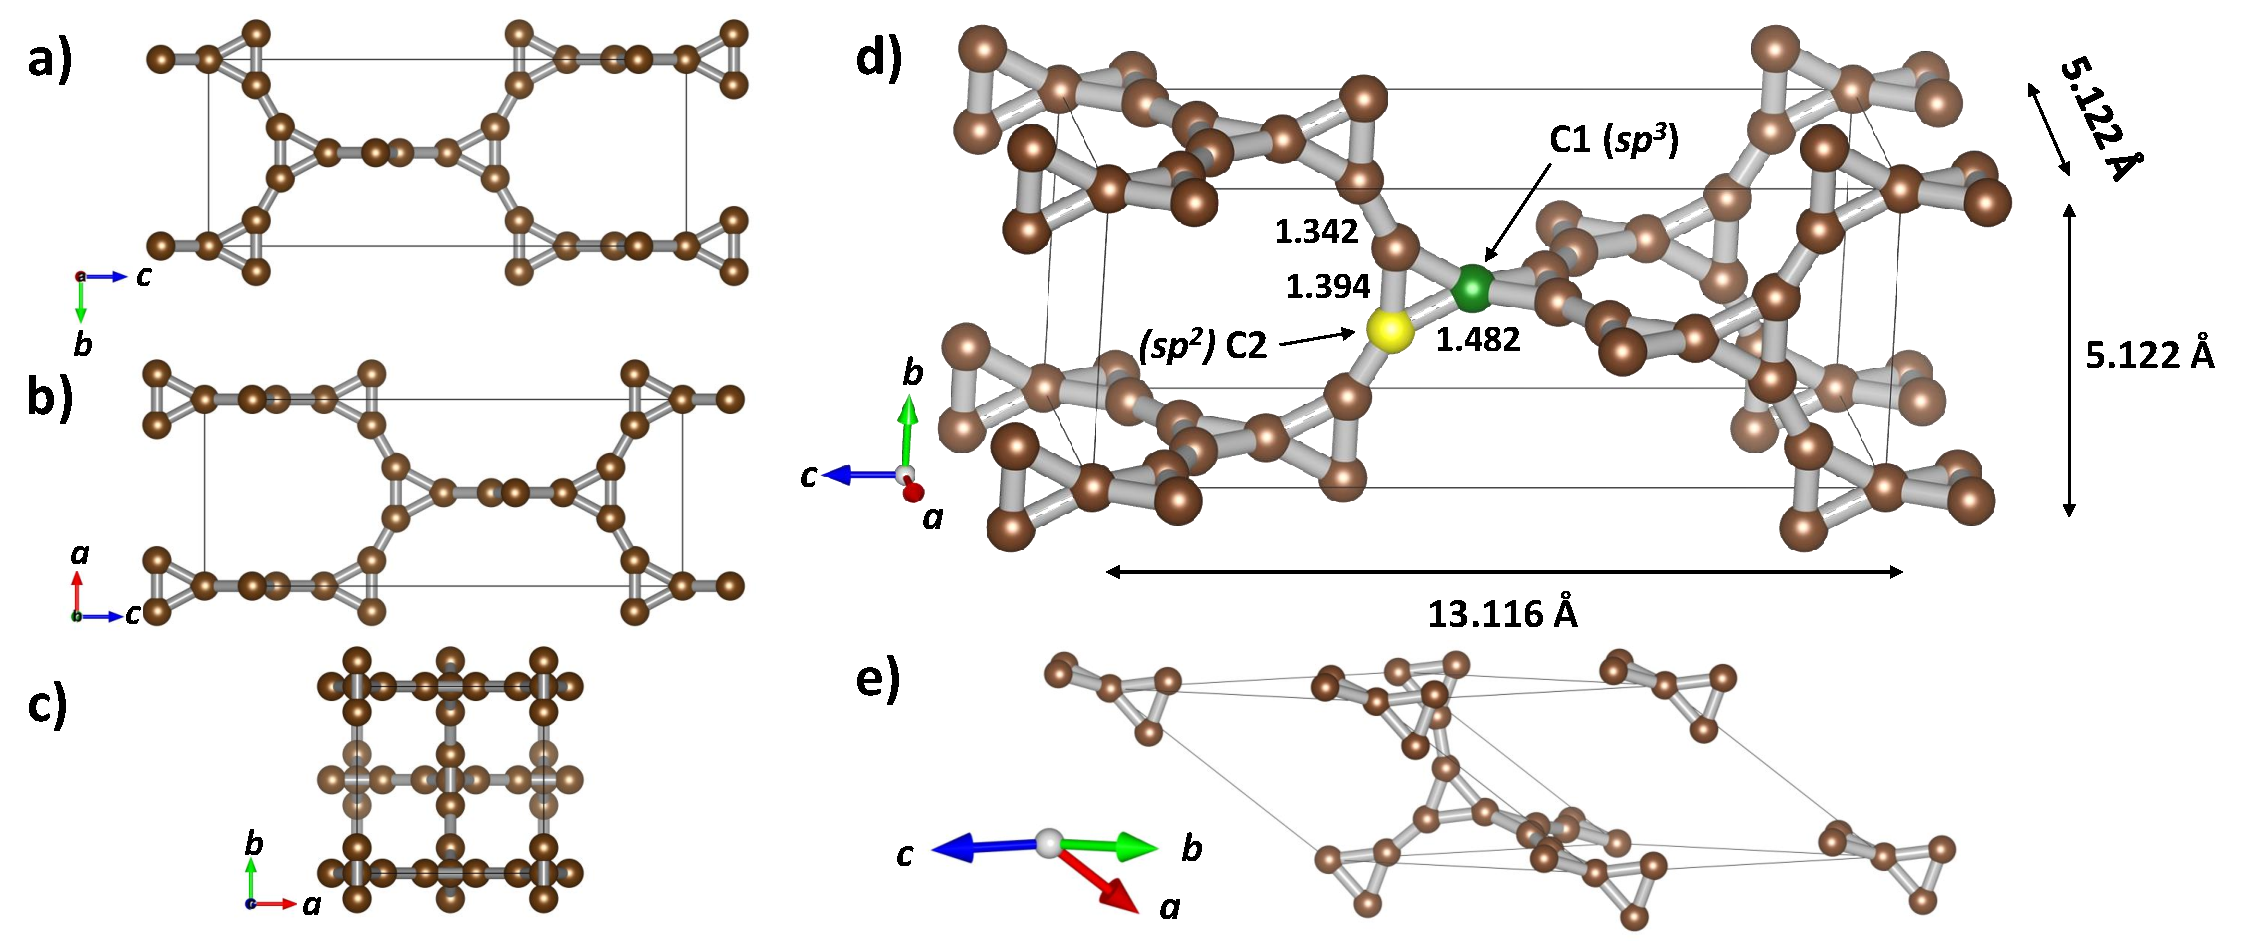
\includegraphics[width=1\linewidth]{capitulos/fig/results1/estrutura_spiro}
		\caption{Representação atômica da estrutura tetragonal do Spiro-Carbon ao longo dos eixos $a$, $b$ e $c$ (\textbf{a)} - \textbf{c)}). \textbf{d)} Representação atômica da estrutura tetragonal do Spiro-Carbon. Por simplicidade é mostrado a célula tetragonal simples, contendo duas fórmulas unitárias por cela. Essa simplificação ajuda no entendimento da estrutura de forma mais intuitiva. \textbf{e)} célula primitiva tetragonal de corpo centrado.}
		\label{estrutura_spiro}
	\end{figure}

	Baseado nos elementos de simetria apresentados pelo Spiro-Carbon, os dois átomos não equivalentes ocupam as posições de Wyckoff \textit{4a} e \textit{16h}, estando \textbf{C1} (destacado em verde) no sítio \textit{4a} com coordenadas fracionárias (0, 0, 0) e \textbf{C2} (destacado em amarelo) no sítio \textit{16h}, com coordenadas fracionárias (0.00000,  0.13609,  0.09971). Analisando a estrutura otimizada é possível distinguir três diferentes tipos de ligação, como representado na \autoref{estrutura_spiro}-d): \textit{i)} As ligações conectando o carbono $sp^3$ central aos seus vizinhos (C1-C2), com comprimento de 1.482 Å, similar às ligações equivalentes na estrutura de seu análogo molecular spiropentadieno\footnote{Os cálculos para a molécula spiropentadieno são apresentadas no \autoref{chap:spiropentadiene}} (que apresenta 1.483 Å) e apresentando comprimento compatível com ligações C-C simples; \textit{ii)} as ligações entre os átomos de carbono $sp^2$ (C2-C2) com comprimento de ligação de 1.394 Å, consideravelmente maior do que a ligação correspondente no spiropentadieno (1.31 Å) e apresentando um caráter intermediário entre ligações simples e duplas, algo típico de ligações duplas conjugadas \cite{lide1962survey}; \textit{iii)} as ligações que conectam os motivos estruturais spiro para formar a estrutura polimérica (C2=C2), com comprimento de ligação de 1.342 \AA, característico de ligações duplas C=C \cite{zavitsas2003relation,lide1962survey}.  
	
	Os ângulos entre os anéis de três membros na porção \textit{spiro} são de 90$^\circ$, mesmo de seu análogo molecular. Os ângulos internos são 62$^\circ$ (C1-C2-C2 e C2-C2-C1) e 56$^\circ$ (C2-C1-C2), levemente diferentes dos apresentados pelo análogo molecular, 63.6$^\circ$ e 52.8$^\circ$ respectivamente. Essa pequena diferença pode ser explicada pelo aumento do comprimentos das ligações endo-anulares (C2-C2), decorrente da formação da estrutura periódica, de forma a aliviar a tensão anular. 
			
	Essa modificação nos comprimentos e ângulos de ligação na porção \textit{spiro}, que resulta da formação da ligação dupla exo-anular em vez da endo-anular como no composto molecular, contribui para uma redução da tensão de anel nesta porção da estrutura e promove um aumento da estabilidade estrutural da forma cristalina. Além disso, essa modificação no perfil das ligações químicas pode gerar consequências interessantes na estrutura eletrônica desse novo alótropo de carbono, como será explorado posteriormente.
	
	Uma forma interessante de visualizar a estrutura do Spiro-Carbon é imaginar esse alótropo como sendo um arranjo perpendicular de fios condutores de \textit{cis}-(poli)acetileno "unidos" por átomos de carbono $sp^3$, como apresentado na \autoref{spiro_fios}.
	
	\begin{figure}[ht]
		\centering
		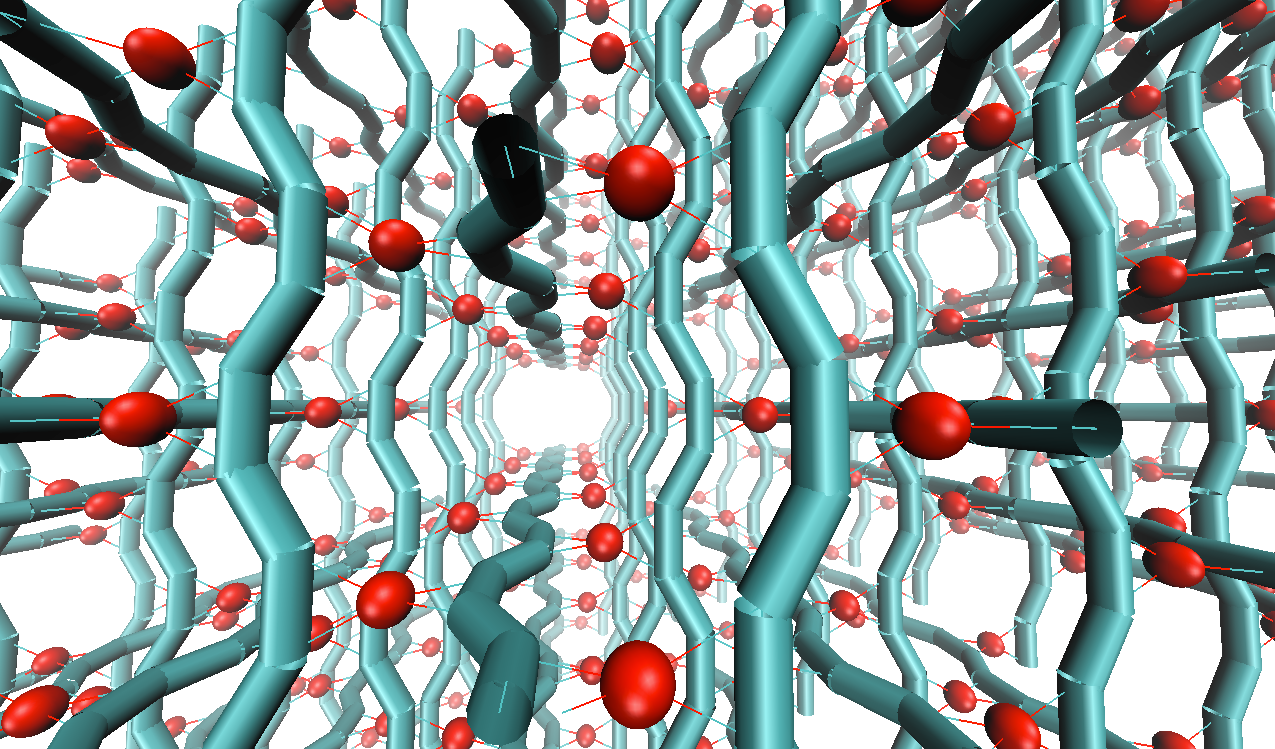
\includegraphics[width=.7\linewidth]{capitulos/fig/results1/column5.png}
		\caption{Representação esquemática do Spiro-Carbon, destacando seu caráter análogo a fios condutores de \textit{cis}-(poli)acetileno "unidos" por átomos de carbono $sp^3$.}
		\label{spiro_fios}
	\end{figure}
	
	\subsection{Estabilidade Relativa e Propriedades Mecânicas}
	
	Para investigar a estabilidade relativa da nova estrutura proposta, foi calculada a dispersão de fônons ao longo de um caminho entre pontos de alta simetria na primeira zona de Brillouin \cite{bradley2010mathematical}. Como pode ser observado na \autoref{phDOS_EoS}-a), nenhuma frequência imaginária foi encontrada, confirmando que a estrutura do Spiro-Carbon corresponde a um mínimo na superfície de energia potencial. 
	
	\begin{figure}[ht]
		\centering
		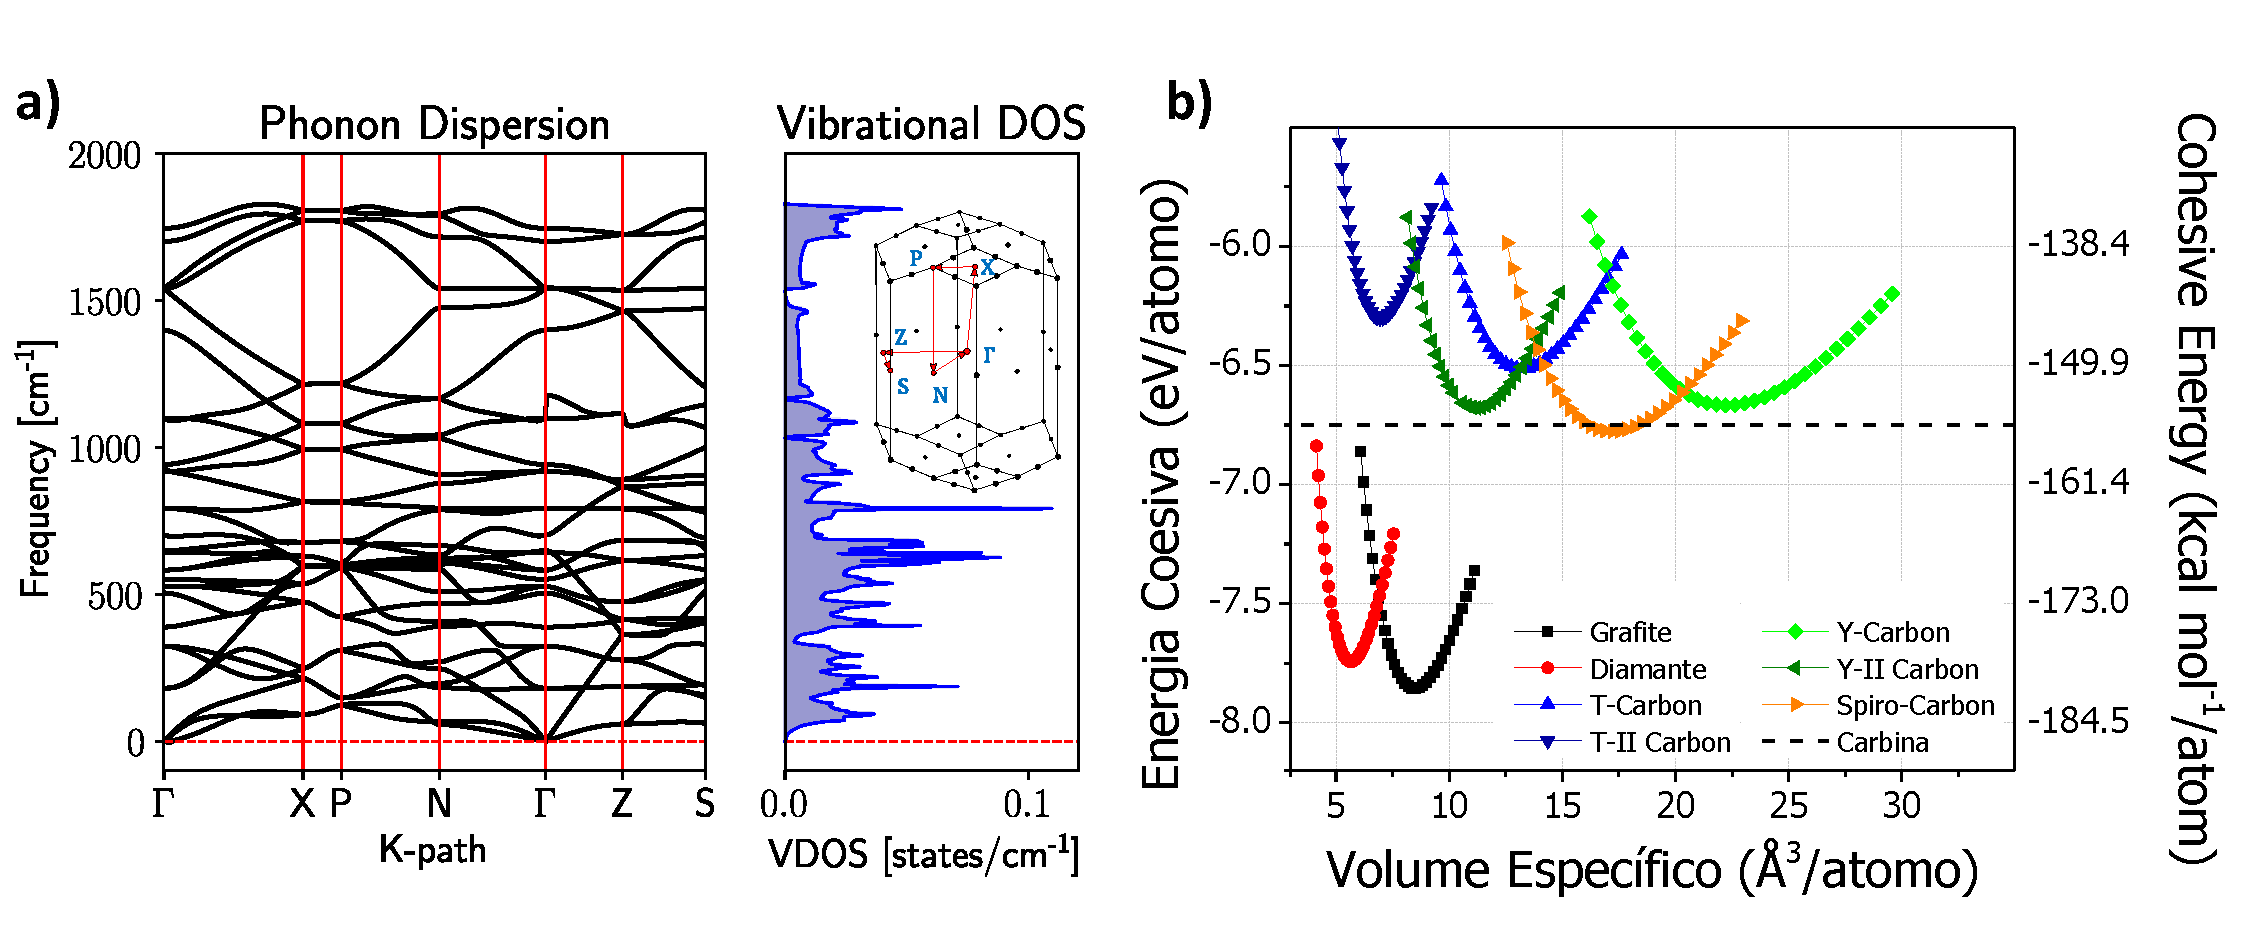
\includegraphics[width=1\linewidth]{capitulos/fig/phDOS_EoS}
		\caption{a) Gráfico da dispersão de fônons ao longo de alguns pontos de alta simetria na primeira zona de Brillouin e a correspondente densidade de estados vibracionais (VDOS). Inserto: Caminho através dos pontos de alta simetria da primeira zona de Brillouin. b) Energia coesiva por átomo em função do volume ($E_c(V)$) por átomo para diferentes alótropos de carbono. do Spiro-Carbon}
		\label{phDOS_EoS}
	\end{figure}

	Para aprofundar o entendimento sobre a estabilidade termodinâmica relativa do Spiro-Carbon, a \autoref{phDOS_EoS}-b) mostra a variação da energia coesiva em função do volume (ambos por átomo) para diferentes alótropos de carbono. Como esperado, a curva $E_c(V)$ para o Spiro-Carbon apresenta claramente um mínimo correspondente ao estado meta estável desta estrutura com menor energia coesiva do que o grafite e o diamante. Apesar disso, o Spiro-Carbon se mostrou mais estável do que outros alótropos de carbono 3D (exceto, é claro, diamante e grafite), como o 1-diamantino/Y-Carbon \cite{costa2018n,li2014modulated}, por aproximadamente 2.3 kcal/mol (0.1 eV) por átomo e o T-Carbon \cite{sheng2011t} por aproximadamente 6.1 kcal/mol (0.26 eV), como mostrado na \autoref{energy}. Esse fato é especialmente encorajador, considerando que recentemente a síntese do T-Carbon foi reportada por \citeauthor{zhang2017pseudo}, utilizando uma suspensão em metanol de nanotubos de carbono \textit{multi-wall} irradiados com laser pulsado em picosegundos.
	
	\begin{table*}[ht]
		\centering
		\renewcommand{\arraystretch}{1.1}
		\caption{Módulo das energias relativa e coesiva por átomo para o Spiro-Carbon comparado com diferentes alótropos de carbono.}
		\label{energy}
		\begin{tabular}{lcccc}
			\hline
			\hline
			\multicolumn{1}{c}{\multirow{2}{*}{Estrutura}} & \multicolumn{2}{c}{Energia Relativa} & \multicolumn{2}{c}{Energia Coesiva}                             \\ \cline{2-5} 
			\multicolumn{1}{c}{}                           & \multicolumn{1}{l}{eV/átomo} & \multicolumn{1}{l}{kcal/mol/átomo} & \multicolumn{1}{l}{eV/átomo} & \multicolumn{1}{l}{kcal/mol/átomo} \\ \hline
				Grafite      & 0.000  & 0.000  & 7.856  & 181.16  \\
				Diamante     & 0.112  & 2.57   & 7.744  & 178.59  \\
				Spiro-Carbon & 1.079  & 24.88  & 6.777  & 156.29  \\
				Carbino      & 1.106  & 25.50  & 6.750  & 155.67  \\
				Y Carbon     & 1.189  & 27.41  & 6.667  & 153.75  \\
				Y-II Carbon  & 1.177  & 27.15  & 6.679  & 154.01  \\
				T Carbon     & 1.342  & 30.94  & 6.514  & 150.22  \\
				T-II Carbon  & 1.554  & 35.84  & 6.302  & 145.32  \\ \hline \hline
		\end{tabular}
	\end{table*}
	
	
	Avaliando agora a estabilidade mecânica da nova estrutura proposta, as seis constantes elásticas ($\textbf{C}_{ij}$ em GPa) foram calculadas e são apresentadas na \autoref{elastic}.
	
	\begin{table}[ht]
		\centering
		\renewcommand{\arraystretch}{1.1}
		\caption{Constantes elásticas ($\textbf{C}_{ij}$ in GPa), módulo Bulk (\textbf{B}), shear (\textbf{G}) e Young (\textbf{E}) (em GPa) e razão de Poisson ($\nu$) calculados para o Diamante, T-Carbon, 1-diamantino (Y-Carbon) e Spiro-Carbon}
		\label{elastic}
		\begin{tabular}{lccccc}
			\hline \hline
			                             & Diamante Exp.\textsuperscript{\cite{grimsditch1975brillouin}}     &Diamante Calc. & T-Carbon & 1-diamantino & Spiro-Carbon \\\hline
			\textbf{C\textsubscript{11}} &  1076.4 $\pm$ 0.2 & 1106.43 & 210.98 & 101.68      & 277.76       \\
			\textbf{C\textsubscript{33}} &	1076.4 $\pm$ 0.2 & 1106.43 & 143.75 & 101.68      & 308.54       \\
			\textbf{C\textsubscript{44}} &  577.4 $\pm$ 1.4  & 591.34  & 66.14 & 13.52       & 75.04        \\
			\textbf{C\textsubscript{66}} &  577.4 $\pm$ 1.4  & 591.34  & 66.14 & 13.52       & 3.61         \\
			\textbf{C\textsubscript{12}} & 	125.2 $\pm$ 2.3  & 153.08  & 143.75 & 79.58       & 3.36         \\
			\textbf{C\textsubscript{13}} &	125.2 $\pm$ 2.3  & 153.08  & 143.75 & 79.58       & 68.88        \\
			\textbf{B}                   &	442.27$\pm$ 1.53 &  470.86 & 166.62 & 86.94       & 123.73       \\
			\textbf{G}                   &	524.68$\pm$ 0.70 &  542.45 & 50.40 & 12.47       & 47.79        \\
			\textbf{E}                   & 1127.98$\pm$ 1.55 & 1175.83 & 137.30 & 35.71       & 121.98       \\
			\textbf{$\nu$}               &  0.075$\pm$ 0.048 &  0.084  & 0.362 & 0.43        & 0.276        \\
			\hline \hline
		\end{tabular}
		\noindent
	\end{table}
	
	As quatro condições necessárias e suficientes que devem ser satisfeitas, baseadas nos critérios de estabilidade de Born \cite{born1940stability}, para garantir a estabilidade mecânica para uma rede tetragonal são:
	
	\begin{equation*}
	C_{11} > |C_{12}|, \quad 2C_{13} < C_{33} (C_{11} + C_{12}),
	\end{equation*}
	\begin{equation*}
	C_{44} > 0, \quad C_{66} > 0
	\end{equation*}
	
	É possível verificar que todas elas são completamente satisfeitas. Adicionalmente, é pode-se examinar outros critérios que devem ser satisfeitos \cite{mouhat2014necessary}: 
	
	\begin{enumerate}
	    \item[(1)] A matriz \textbf{C} é positiva definida \footnote{Em álgebra linear, uma matriz definida positiva é uma matriz que, em muitos aspectos, é análoga a um número real positivo. A noção é parecida com a de uma forma bilinear simétrica positiva-definida (ou uma forma sesquilinear no caso complexo). A definição adequada de definida positiva não tem ambiguidades no caso de matrizes Hermitianas, mas não há consenso na literatura a respeito de como ela deve ser estendida para matrizes não Hermitianas, se é que isso deve ser feito.} ;
	    \item[(2)] Todos os autovalores de \textbf{C} são positivos;
	    \item[(3)] Todos os menores principais de \textbf{C} \footnote{determinantes das \textit{k} submatrizes da esquerda superior,para 1 $\leq$ \textit{k} $\leq$ 6} são positivos  (critério de Sylvester); e
	    \item[(4)] Um conjunto arbitrário de menores de \textbf{C} são positivos. 
	\end{enumerate}

	Todos esses critérios são satisfeitos pelo Spiro-Carbon, dessa forma podemos concluir que essa nova estrutura proposta é mecanicamente estável. 
	
	Para caracterizar o comportamento mecânico no regime elástico desta nova estrutura, uma análise tensorial completa da matriz elástica foi conduzida. Os valores médios das principais propriedades mecânicas foram calculadas segundo três diferentes métodos de aproximação e são apresentadas na \autoref{average_elastic}.
	
	\begin{table*}[!ht]
		\centering
		\renewcommand{\arraystretch}{1.5}
		\caption{Valores médios das principais propriedades mecânicas do Spiro-Carbon.}
		\label{average_elastic}
		\begin{tabular}{@{}ccccc@{}}
			\hline
			\hline
			Aproximação & Módulo     & Módulo de   & Módulo      & Razão de \\ 
			            & Bulk (GPa) & Young (GPa) & Shear (GPa) & Poisson \\ \hline
			Voigt       & 127.37 & 196.25 & 78.93 & 0.24 \\
			Reuss       & 124.06 &  44.86 & 15.58 & 0.44 \\
			Hill        & 125.71 & 125.98 & 47.25 & 0.33 \\\hline
			\hline
		\end{tabular}
	\end{table*}

	
	\begin{figure*}[!ht]
		\centering
		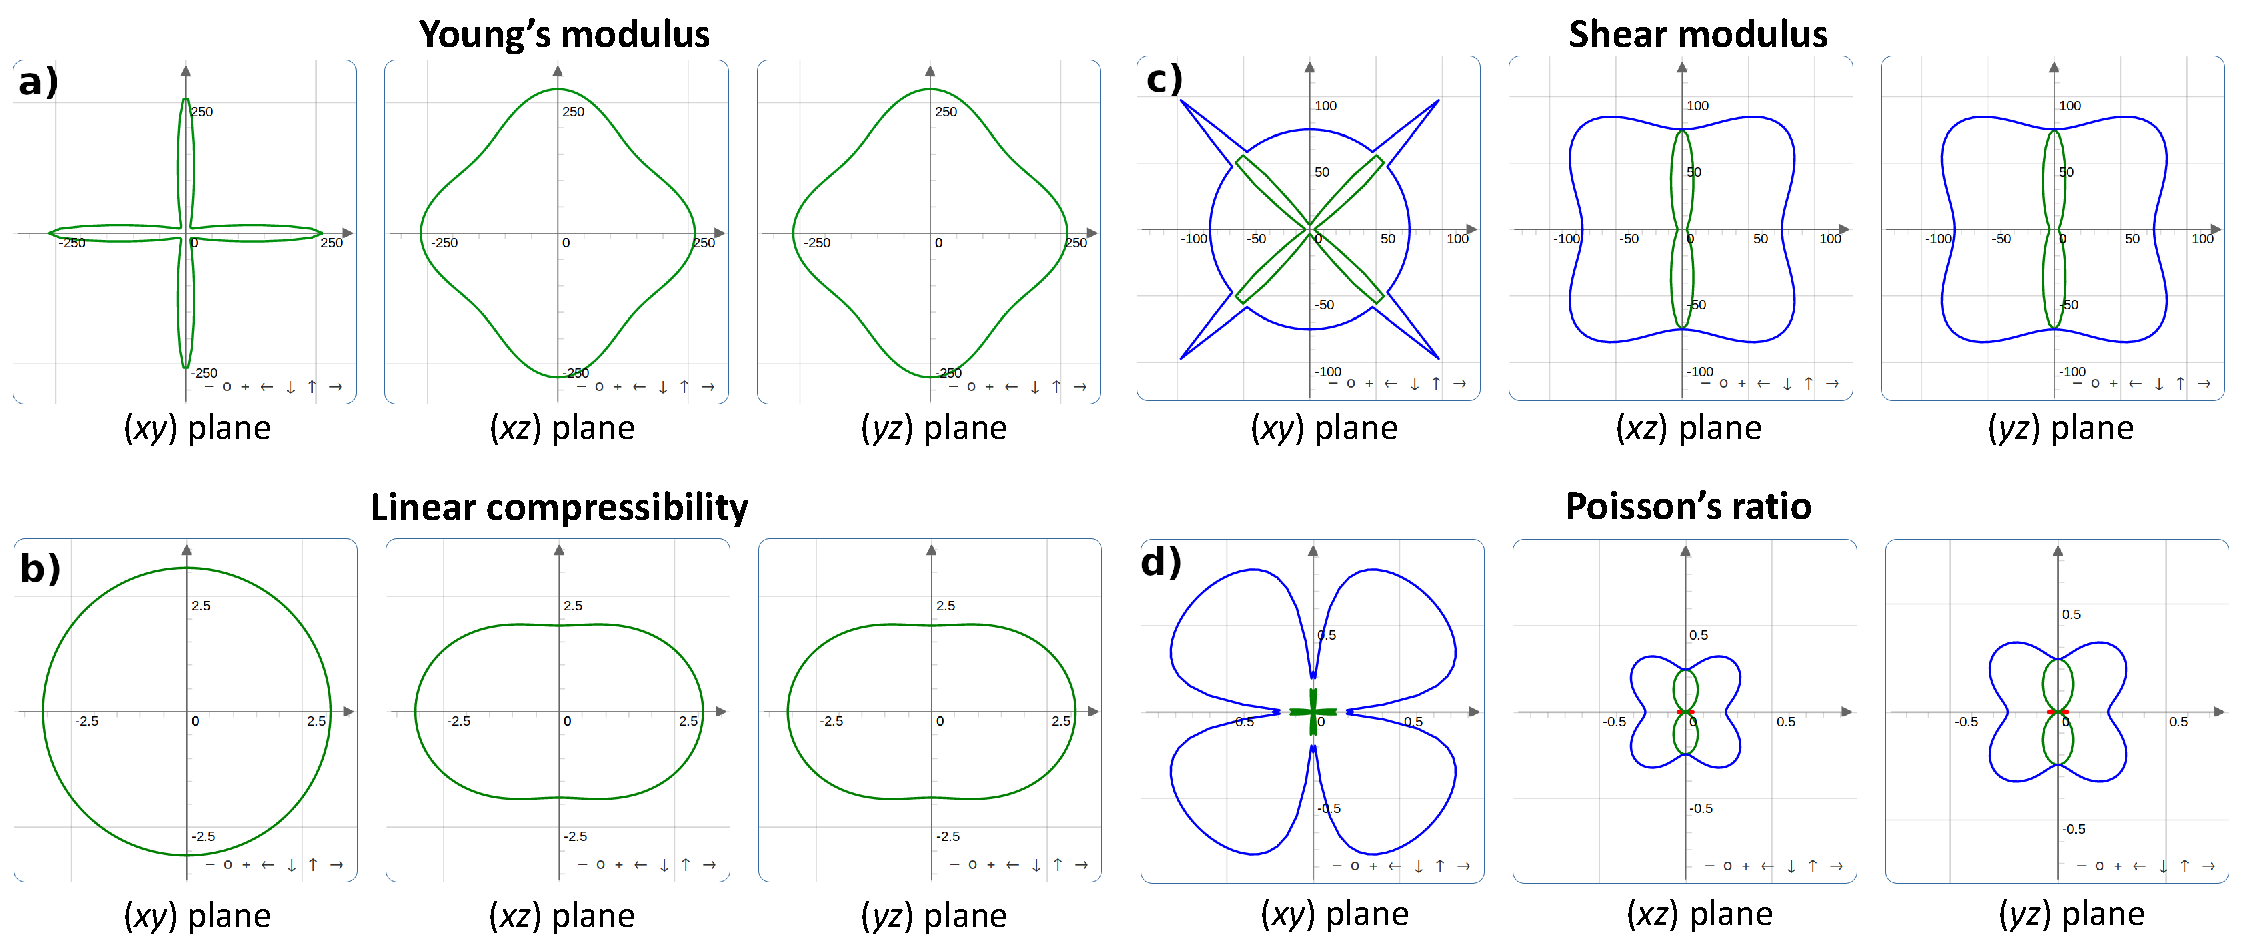
\includegraphics[width=1\linewidth]{capitulos/fig/elastic_2}
		\caption{Dependência espacial do (a) módulo de Young; (b) compressibilidade linear; (c) módulo Shear e (d) razão de Poisson.}
		\label{elastic_m}
	\end{figure*}
	
	A \autoref{elastic_m} mostra os gráficos da dependência espacial nos planos \textbf{xy}, \textbf{xz} e \textbf{yz} para os módulos de Young (\textbf{E}) e shear  (\textbf{G}), compressibilidade linear  ($\beta$) e razão de Poisson ($\nu$). A principal característica que podemos destacar é a grande anisotropia no plano \textbf{xy} para todas as propriedades, exceto a compressibilidade linear. Essa característica é comum para materiais porosos \cite{ortiz2012anisotropic} e pode ser um grande indicativo de que o Spiro-Carbon, quando sintetizado, se apresentará como um material altamente dúctil. 
	
	A anisotropia do módulo de Young, caracterizada pela razão A\textsubscript{E} = E\textsubscript{max}/E\textsubscript{min} é de 19.58. Os valores máximos dessa propriedade coincidem com as direções dos eixos \textit{x}, \textit{y} e \textit{z}, exibindo valor máximo de 274.78 GPa nessas direções. Em todas as outras direções do plano \textit{xy} os valores apresentados são excepcionalmente baixos, possuindo valore mínimo de 14.03 GPa. O módulo de cisalhamento, também conhecido como módulo de rigidez ou módulo de torção, também apresenta a mesma tendência, possuindo alta anisotropia, A\textsubscript{G} = 29.98, mas com seus valores máximos nas direções diagonais aos planos \textit{xy}, \textit{xz} e \textit{yz}. Os valores médios de todas as propriedades calculadas são apresentadas na \autoref{average_elastic}.
	
	Uma boa maneira de avaliar a dureza que o material policristalino poderia ter é utilizando o modelo empírico de \citeauthor{chen2011modeling}. Utilizando esse modelo, a dureza de Vicker obtida para o Spiro-Carbon é de 4,37 GPa (446 HV)\footnote{1 HV = 0.009807 GPa} valor muito mais baixo do que o para o diamante (90,9 GPa, 9266 HV) porém acima do apresentado pelo T-Carbon (1,89 GPa, 193 HV). Esse baixo valor de dureza indica que, uma vez sintetizado, esse material irá pertencer à classe de materiais maleáveis, uma característica interessante considerando a demanda crescente pelo desenvolvimento de materiais condutores e maleáveis \cite{kim2008stretchable, valentine2017hybrid, gong2017one}.
	%
	
	\subsection{Propriedades Eletrônicas}
	
	Como mencionado anteriormente, a estrutura do Spiro-Carbon se assemelha a um conjunto cadeias de \textit{trans-cisoide}-(poli)acetileno nos eixos \textit{x} e \textit{y} interconectados por átomos de carbono com hibridação $sp^3$. Uma vez que a cadeia de \textit{trans-cisoide}-(poli)acetileno isolada é um semi-condutor com \textit{band gap} de aproximadamente 1.3 eV \cite{baughman1982structural}, seria razoável imaginar que a estrutura eletrônica do Spiro-Carbon herdasse essa característica. Curiosamente ao analisar o diagrama de bandas, apresentado na \autoref{band1}, é possível observar que o Spiro-Carbon apresenta um caráter eletrônico metálico, devido à interseção entre as bandas de condução e de valência abaixo do nível de Fermi próximo ao ponto Z da zona de Brillouin. 
	
	
	\begin{figure}[!ht]
		\centering
			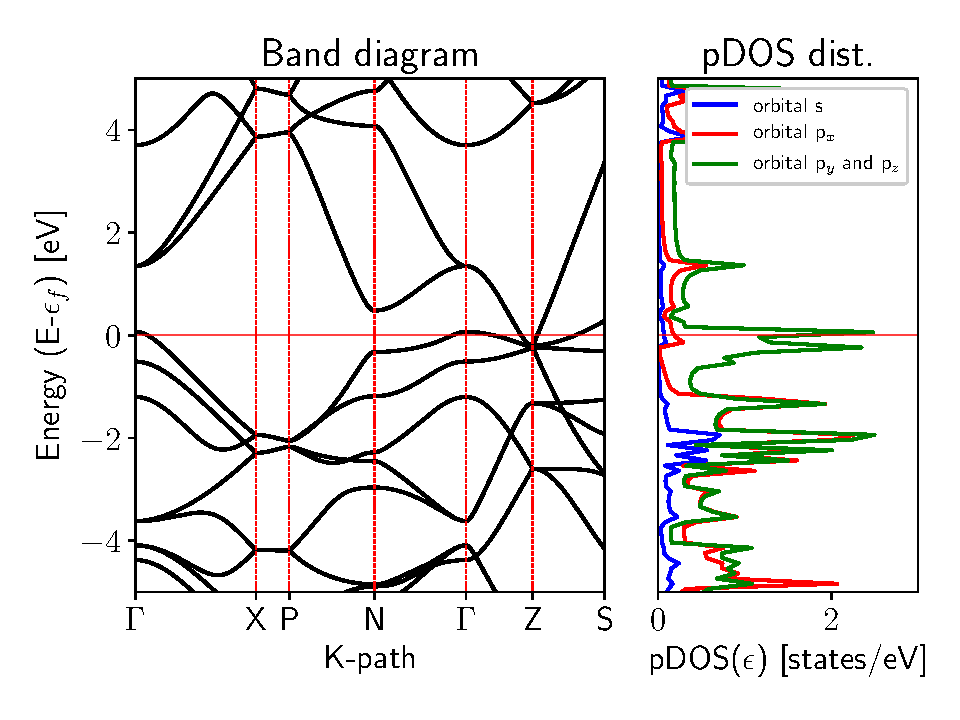
\includegraphics[width=.8\linewidth]{capitulos/fig/results1/bands_smearing}
		\caption{Dispersão de energia das bandas ao longo dos principais pontos de alta simetria na primeira zona de Brillouin (esquerda) e densidade de estados projetada nos orbitais (direita) para o Spiro-Carbon. A energia de Fermi ($\epsilon_f$) foi ajustada para 0.}
		\label{band1}
	\end{figure}

	A \autoref{pdos_byatom} apresenta a densidade de estados projetada (pDOS) referente a cada átomo que compõe a célula primitiva. É possível observar que o átomo \textbf{C2}, com hibridação $sp^2$ é o único que apresenta contribuição para a densidade de estados próxima do nível de Fermi. Isso pode ser um forte indicativo de que as ligações duplas conjugadas formadas por esses átomos sejam as principais responsáveis pelo caráter metálico deste material. 
	
	
	\begin{figure}[!ht]
		\centering
		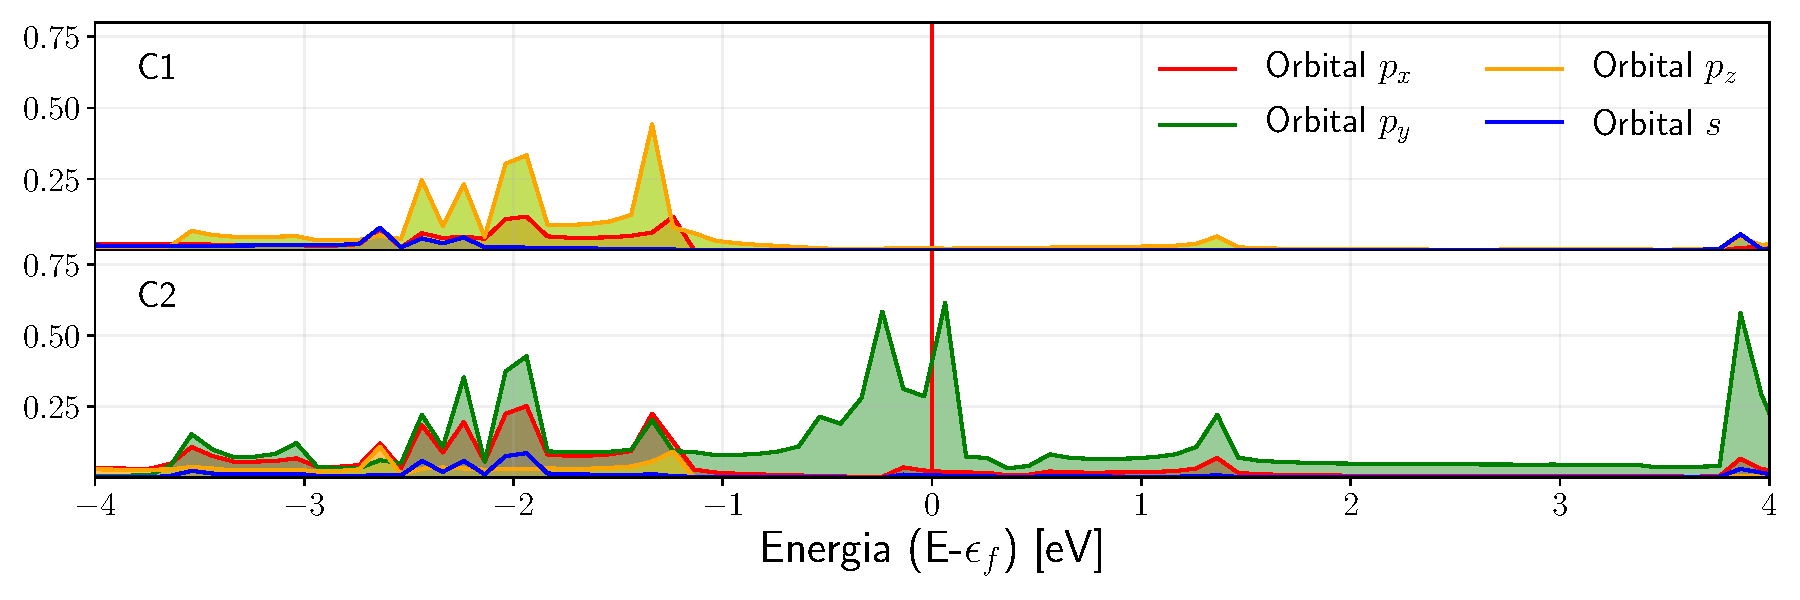
\includegraphics[width=1.\linewidth]{capitulos/fig/results1/pdos_byatom0}
		\caption{Densidade de estados projetada para cada átomo da célula primitiva. Em cima para o átomo \textbf{C1} e em baixo para o átomo \textbf{C2}. A energia de Fermi ($\epsilon_f$) foi ajustada para 0.}
		\label{pdos_byatom}
	\end{figure}


	É apresentado na literatura que a cadeia de \textit{trans-}(poli)acetileno seria condutora se todas as ligações entre os átomos de carbono tivessem o mesmo comprimento, de 1,391 Å, gerando assim uma cadeia infinita de ligações $\pi$ conjugadas. \cite{suhai1983bond, whangbo1979conjugated} De fato, cálculos feitos no mesmo nível dos apresentados até aqui confirmaram isso (Apêndice \ref{chap:bands_poliacetileno} - \autoref{bands_trans}). O caráter semi-condutor das cadeias de \textit{trans}-(poli)acetileno surgem do fato de que, em uma cadeia unidimensional infinita, o estado fundamental duplamente degenerado é instável devido à \textit{instabilidade de Peierls}\cite{peierls1996quantum}. Isso faz com que as ligações entre os átomos de carbono alternem entre simples e duplas, quebrando essa degenerescência e forçando os átomos de carbono a se agruparem em pares. Esse fenômeno, conhecido como \textbf{distorção de Peierls}, quebra a simetria translacional e separa os níveis de energia das bandas de valência e condução, convertendo a estrutura em um semi-condutor. \cite{peierls1996quantum}
	
	O \textit{cis}-(poli)acetileno apresenta o mesmo fenômeno, entretanto a distorção das ligações pode gerar duas formas: \textit{cis-transoide}-(poli)acetileno e \textit{trans-cisoide}-(poli)acetileno. Essas duas formas apresentam características eletrônicas parecidas, porém com \textit{band gap} diferentes. As formas \textit{cis}-(poli)acetileno e \textit{cis-transoide}-(poli)acetileno apresentam \textit{band gaps} de 0,8 eV, calculados com funcional PBE, enquanto a forma \textit{trans-cisoide}-(poli)acetileno apresenta band gap de 0,3 eV (para mais detalhes ver \autoref{chap:bands_poliacetileno}).
	
	Na estrutura do Spiro-Carbon as ligações conectando os átomos C2 apresentam comprimento de ligação de 1.342 Å e 1.394 Å, muito próximo dos apresentados pelo \textit{trans-cisoid}-(poli)acetileno, no qual as ligações correspondentes apresentam comprimentos de 1.377 Å e 1.424 Å. Esses valores estão de acordo com observações experimentais e cálculos teóricos reportados na literatura \cite{chien1982estimate, chien2012polyacetylene, whangbo1979conjugated}.
	
	\begin{figure}[!ht]
		\centering
		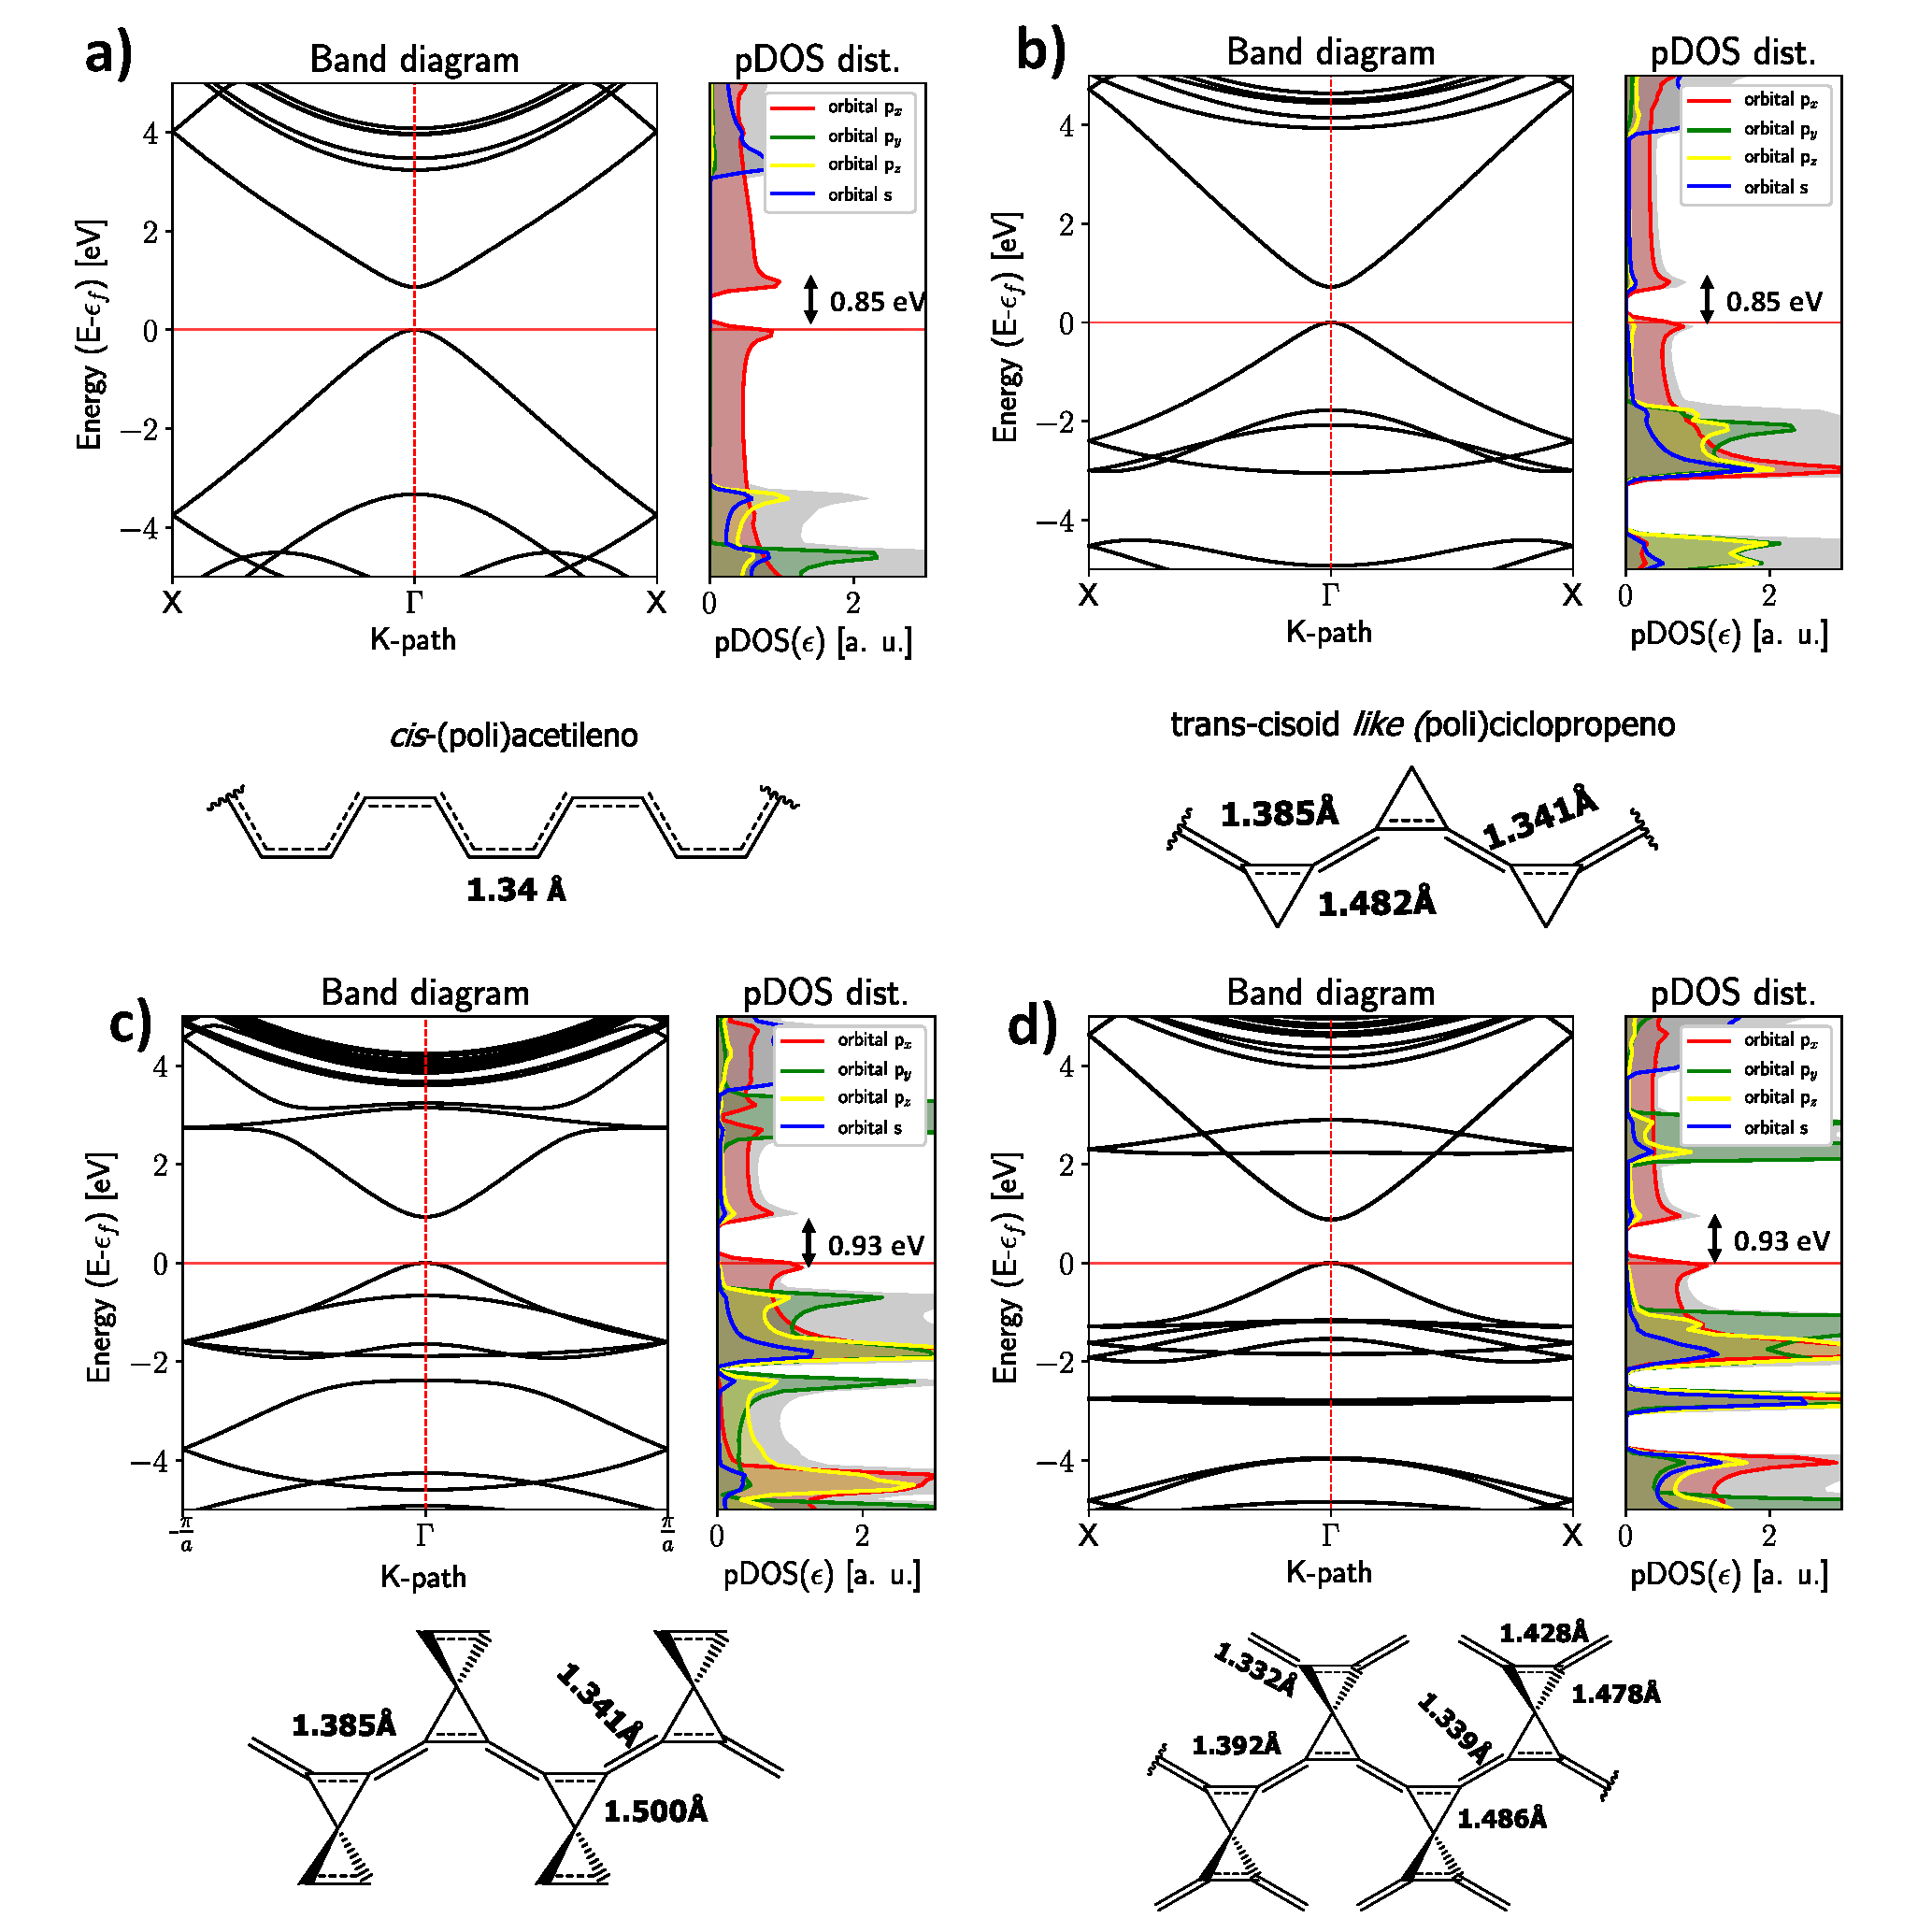
\includegraphics[width=.9\linewidth]{capitulos/fig/results1/poliacetileno_2_spiro}
		\caption{Diagrama de bandas das estruturas intermediárias entre o \textit{cis}-(poli)acetileno e o Spiro-Carbon}
		\label{acetileto_2_spiro}
	\end{figure}

	A \autoref{acetileto_2_spiro} apresenta o diagrama de bandas das estruturas intermediárias entre o \textit{cis}-(poli)acetileno e o Spiro-Carbon. É possível observar que conforme a cadeia lateral aumenta e se aproxima da forma estrutural do Spiro-Carbon, os orbitais $p_y$ e $p_z$ começam a apresentar densidades de estados cada vez mais próxima do nível de Fermi, com os orbitais preenchidos "subindo" em energia e os orbitais vazios "descendo" em energia, tendo como caso limite o Spiro-Carbon em que esses orbitais se intersectam. 


	\begin{figure}[!ht]
		\centering
		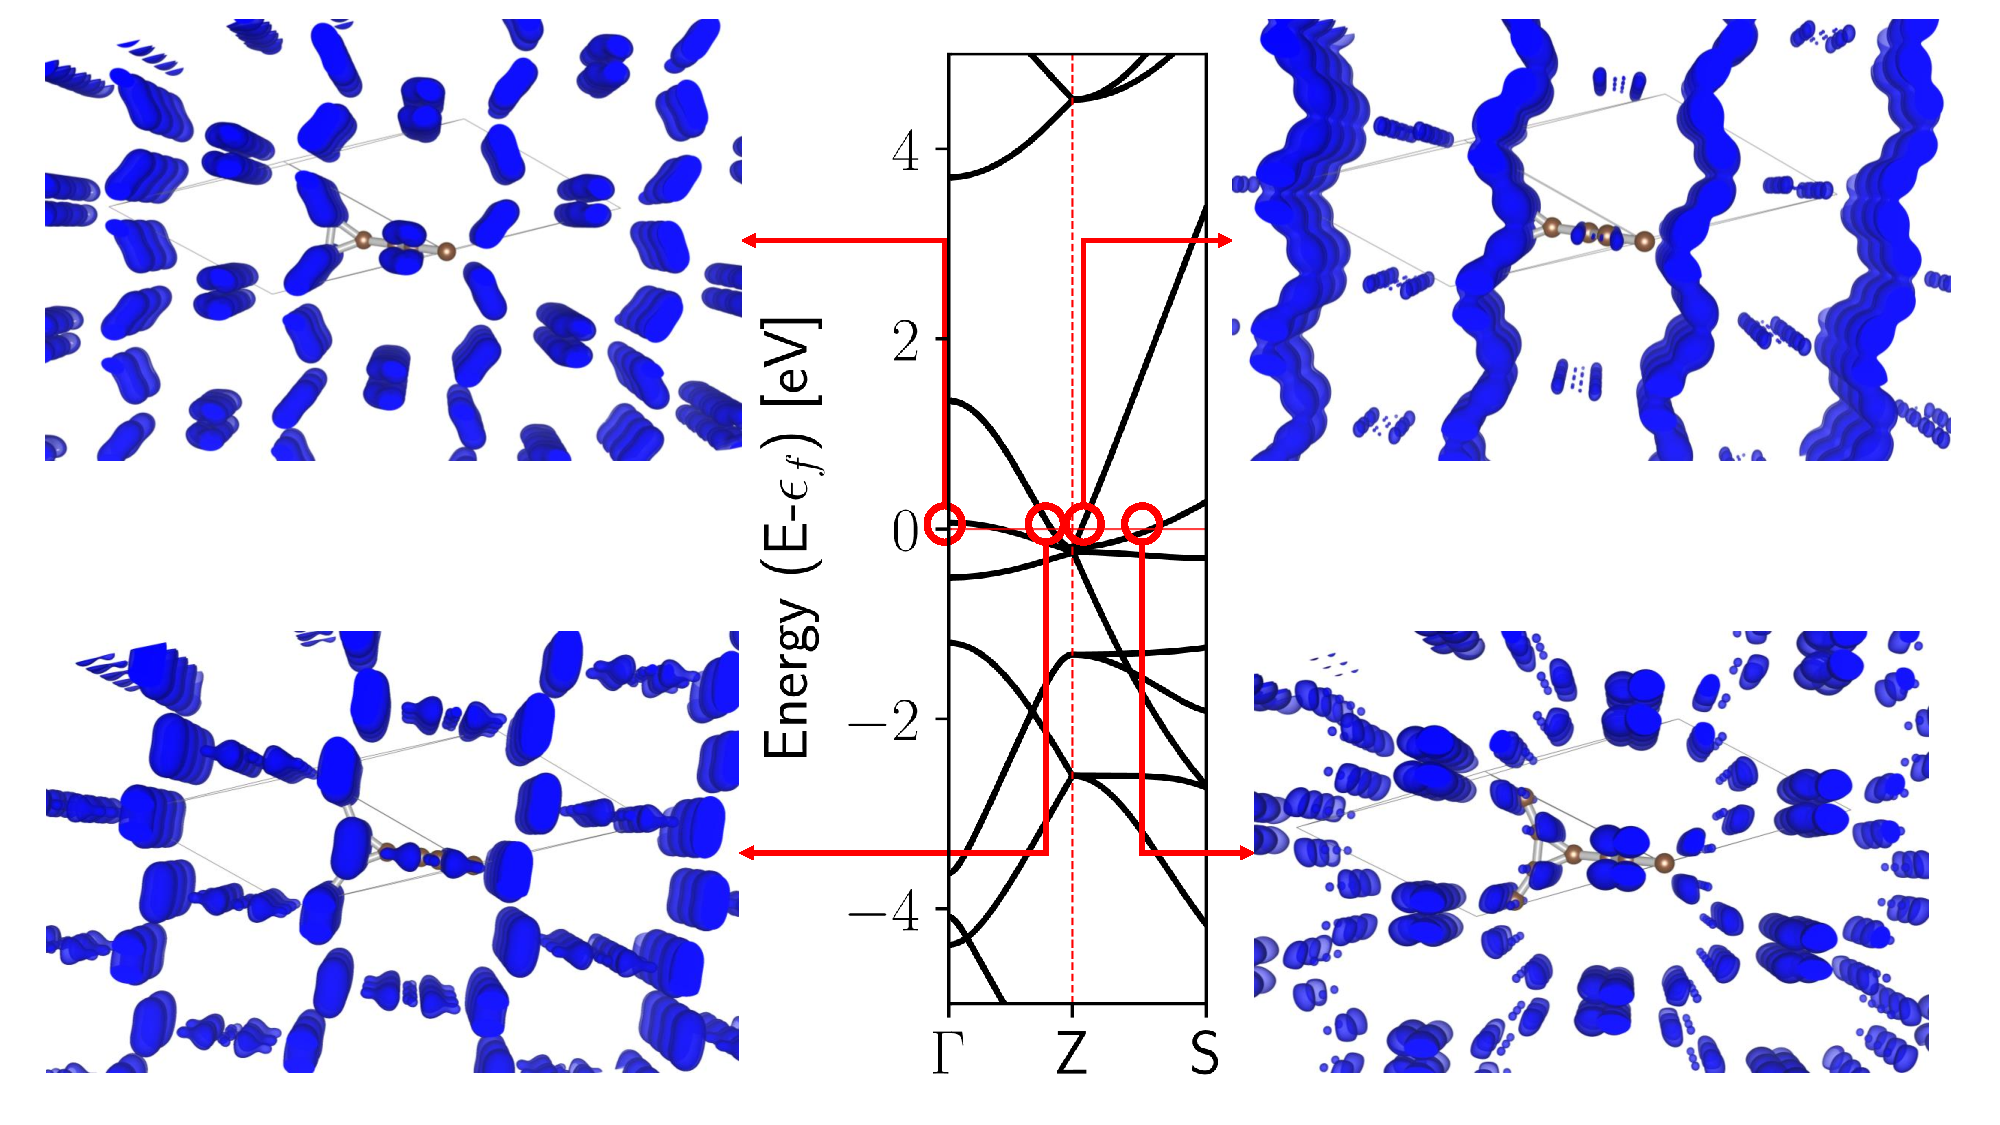
\includegraphics[width=1\linewidth]{capitulos/fig/results1/bands_fermi}
		\caption{Gráfico da (pseudo)-densidade de carga decomposta nas bandas que cruzam o nível de Fermi para a cela primitiva tetragonal. Iso-superfícies ajustadas para 0.005 $a_0^{-3}$, onde $a_0$ é o raio de Bohr.}
		\label{bandas_fermi}
	\end{figure}

	O caráter metálico da estrutura do Spiro-Carbon pode ser entendido qualitativamente, portanto, da seguinte maneira: se a estrutura fosse composta somente das cadeias de \textit{trans-cisoid}-(poli)acetileno, a estrutura seria um semicondutor. De fato, a diferença de energia entre as bandas de valência e condução em $\Gamma$ é de 1.28 eV, valor próximo do \textit{band gap} calculado para a cadeia de \textit{trans}-(poli)acetileno isolada. Entretanto, a interconexão entre as cadeias criada pelo átomo de carbono $sp^3$ gera uma sobreposição das bandas de valência e condução próximo ao ponto Z. Como consequência, bolsões de buracos\footnote{Quasi-partículas equivalentes ao elétron, porém com carga contrária. Corresponde à abstenção de um elétron de um estado abaixo do nível de Fermi.} surgem próximo do topo da banda de valência em $\Gamma$ e a banda de condução passa a ser populada próximo de Z. Dessa forma, podemos ver o caráter metálico da estrutura do Spiro-Carbon como resultante de uma \textit{"dopagem intrínseca"}, ou uma \textit{auto-dopagem}, gerada pela adição do carbono $sp^3$ na estrutura. Ou seja, parece ser possível dopar um determinado elemento com a adição de átomos do mesmo elemento, deste que este apresente hibridação diferente dos demais átomos na estrutura não dopada.    
		
	\begin{figure}[!ht]
		\centering
		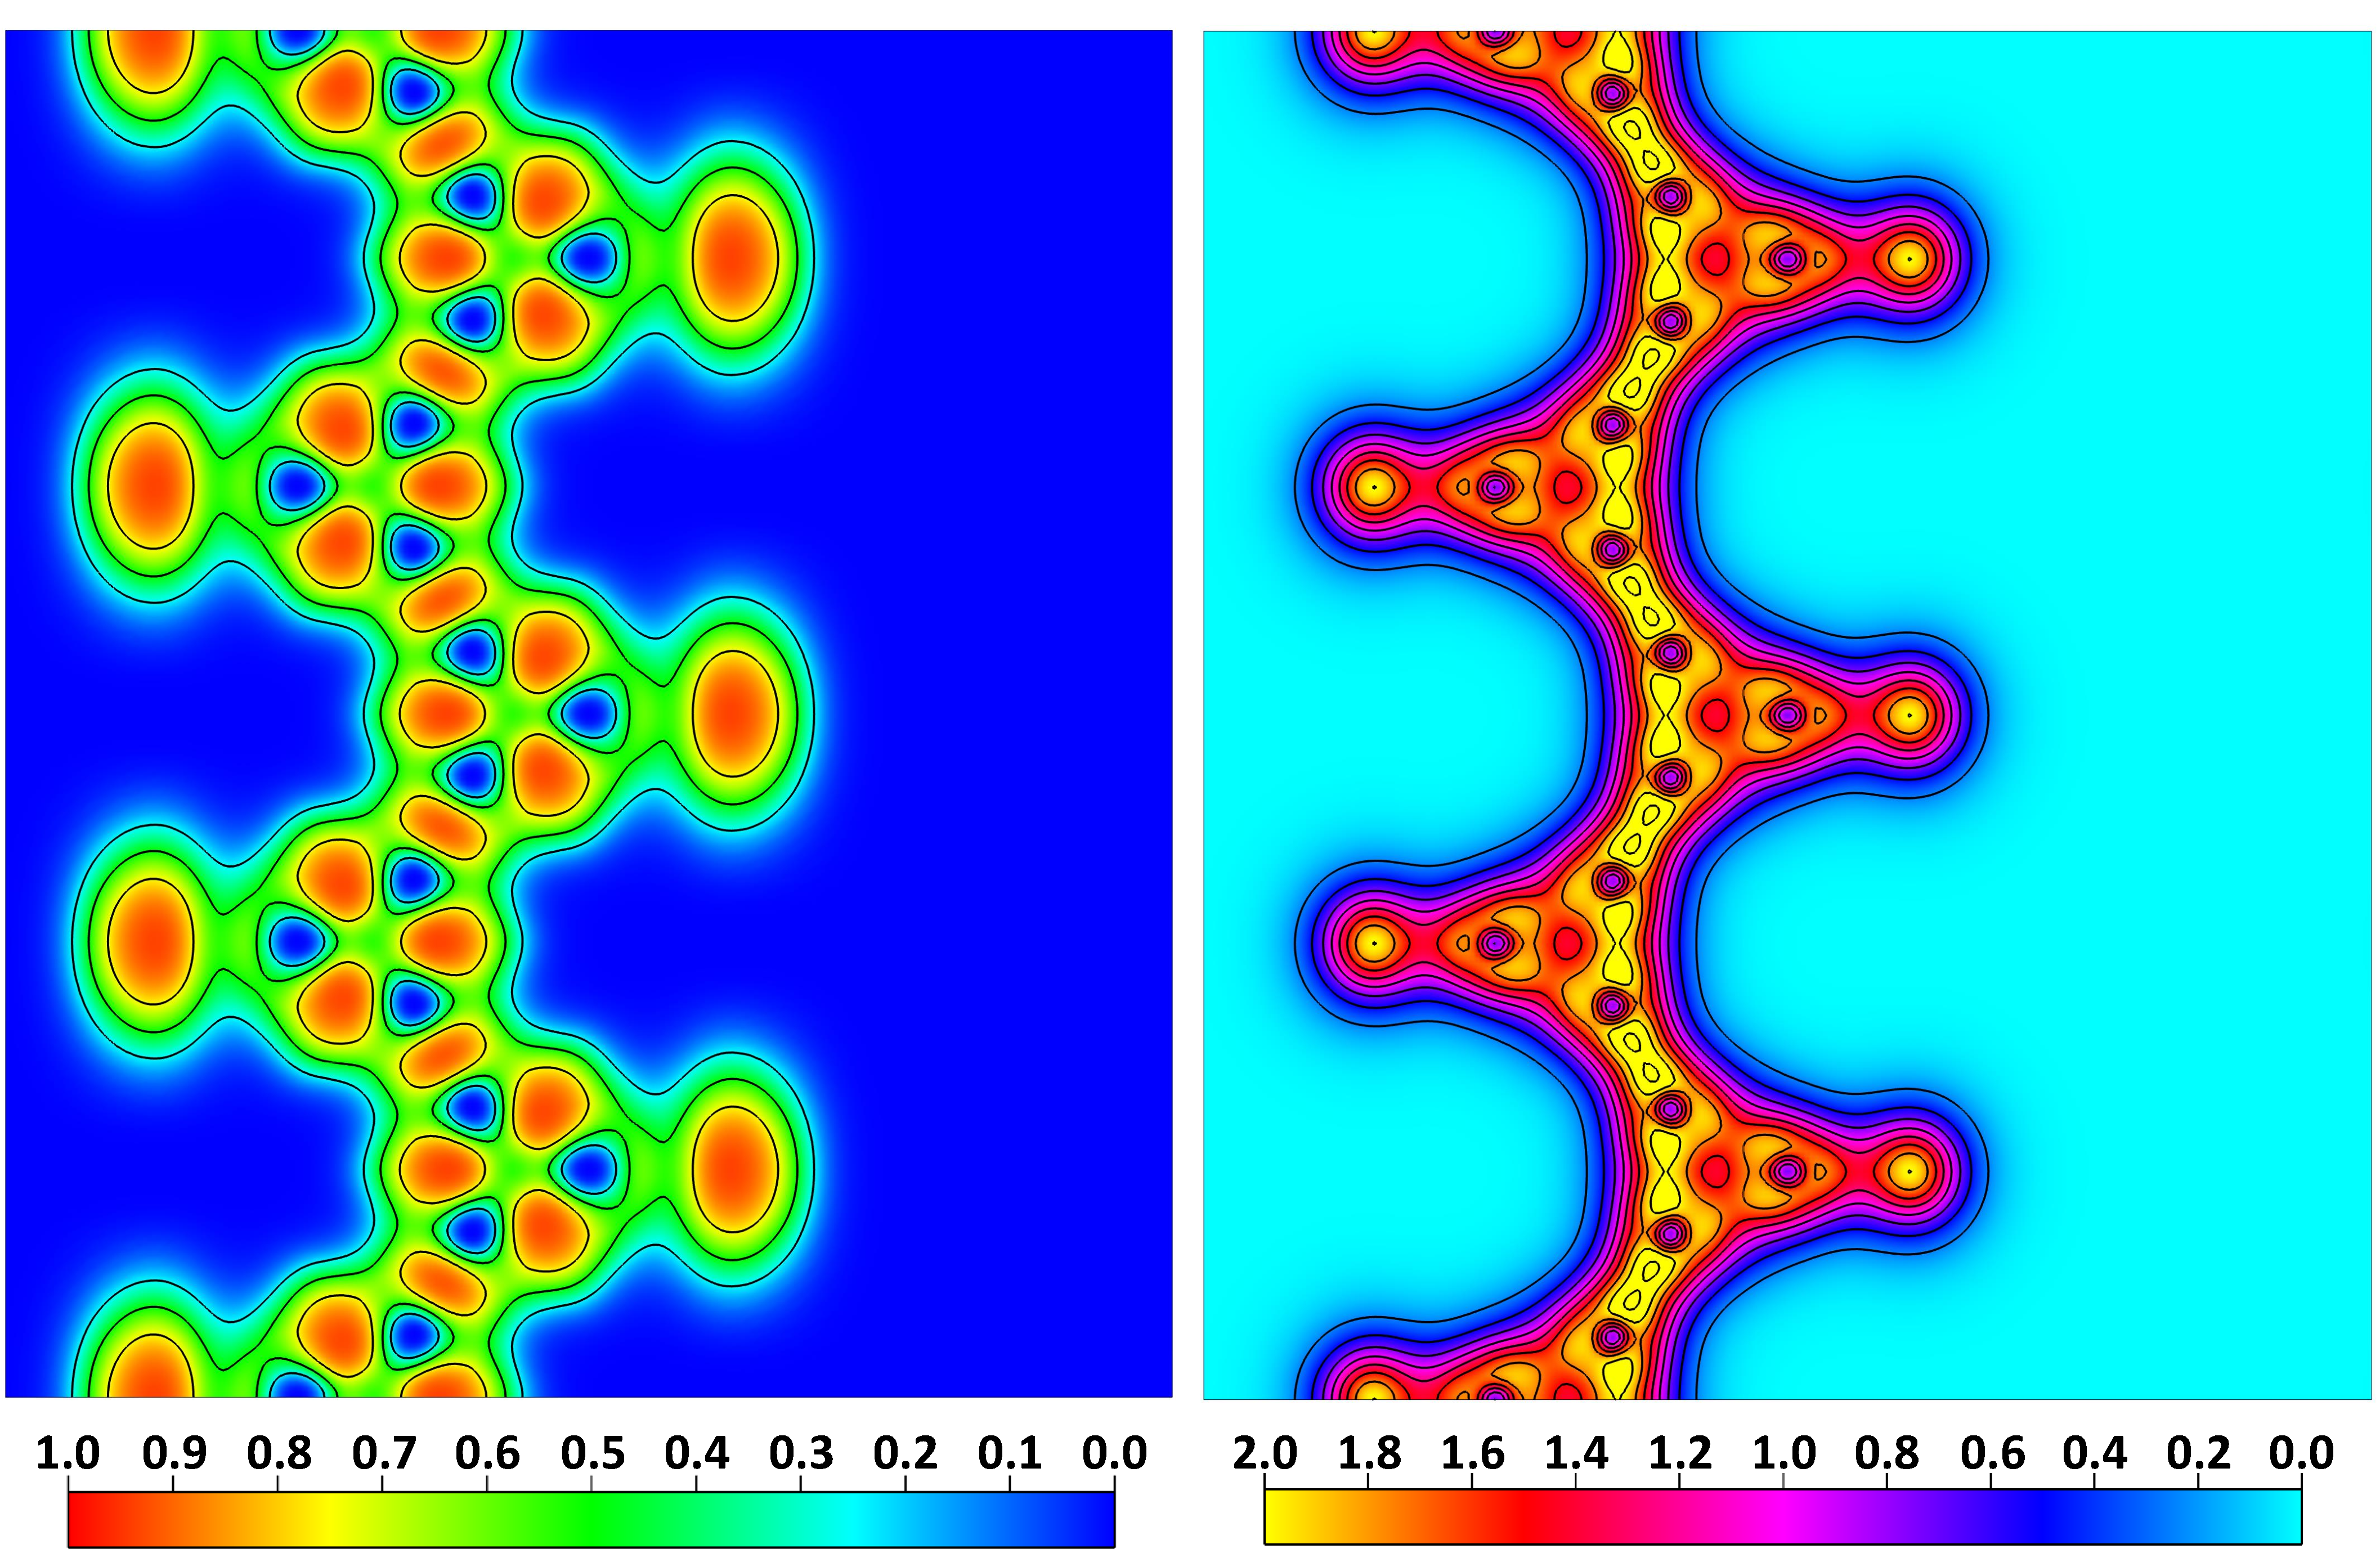
\includegraphics[width=1\linewidth]{capitulos/fig/ELF}
		\caption{À esquerda, o gráfico da função de localização eletrônica no plano (010) da cela tetragonal convencional. As linhas de contorno estão linearmente distribuídas em intervalos de 0,25. À direita, o gráfico da pseudo-densidade de carga no plano (010) da cela tetragonal convencional. A escala apresenta valores entre 0 e 2 e/Å\textsuperscript{3} e as linhas de contorno estão linearmente distribuídas em intervalos de 0,25 e/Å\textsuperscript{3}. Em ambos os casos 3 unidades de repetição no eixo $x$ foram utilizada para facilitar a visualização.}
		\label{elf}
	\end{figure}

	De fato, as iso-superfícies da (pseudo)-densidade de carga para as bandas que cruzam o nível de Fermi confirmam que essas bandas apresentam um claro caráter de orbitais $\pi$ conjugados, reforçando a ideia de que essas ligações deslocalizadas são as principais responsáveis pelo caráter eletrônico metálico da estrutura.  
	
	Esses grandes picos de densidades de estado, remanescentes do caráter \textit{quasi}-1D das cadeias condutoras, sugere que o Spiro-Carbon é um bom condutor que poderá apresentar uma grande anisotropia na condutividade, sendo alta ao longo das direções $xy$ e baixa na direção $z$. Além disso, a alta densidade de estados próximo ao nível de Fermi sugere que o Spiro-Carbon possa apresentar diversos eletrônicos interessantes como magnetismo, supercondutividade, ondas de portadores de carga, dentre outras.

	Por fim, para explorar o grau de deslocalização da estrutura eletrônica a \autoref{elf} apresenta o gráfico da ELF no plano (010) para a cela tetragonal convencional do Spiro-Carbon. É possível observar claramente a alta localização da densidade de carga, com  $\chi_{ELF}>0,75$, entre todos os átomos de carbono referente à ligação $\sigma$ entre esses átomos. Adicionalmente, uma densidade de carga com $0,75\geq \chi_{ELF}\geq 0,25$ pode ser observada se espalhando por toda a estrutura, revelando a natureza altamente deslocalizada da densidade de carga advinda das ligações $\pi$. 
	
	\subsection{Possíveis abordagens sintéticas}
	
	Uma possível rota de síntese para o Spiro-Carbon pode ser proposta derivadas do acoplamento de Suzuki-Miyaura entre unidades do spiropentadieno halogenadas contendo grupos éster borônico, como apresentado na \autoref{synthesis}. Os precursores poderiam ser obtidos através da química de carbenos ou por estratégias comparáveis às empregadas por \citeauthor{billups1991spiropentadiene}.
	
	\begin{figure}[!ht]
		\centering
		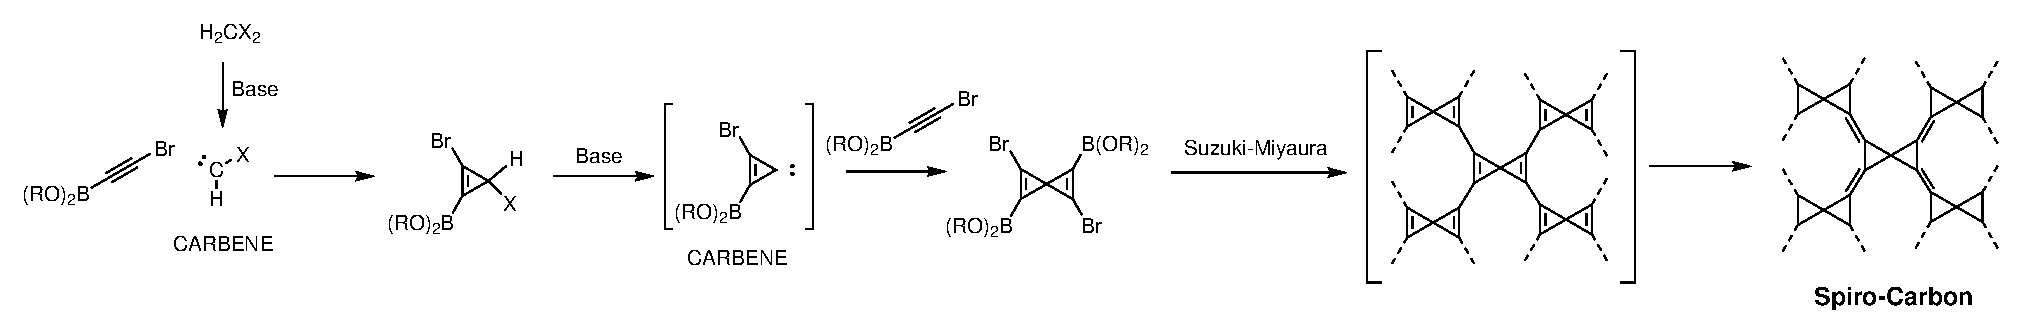
\includegraphics[width=1.\linewidth]{capitulos/fig/results1/synthesis_polyspiro1.eps}
		\caption{Possível rota sintética para a obtenção do Spiro-Carbon}
		\label{synthesis}
	\end{figure}


	\begin{figure}[ht]
		\centering
		\subfloat{
			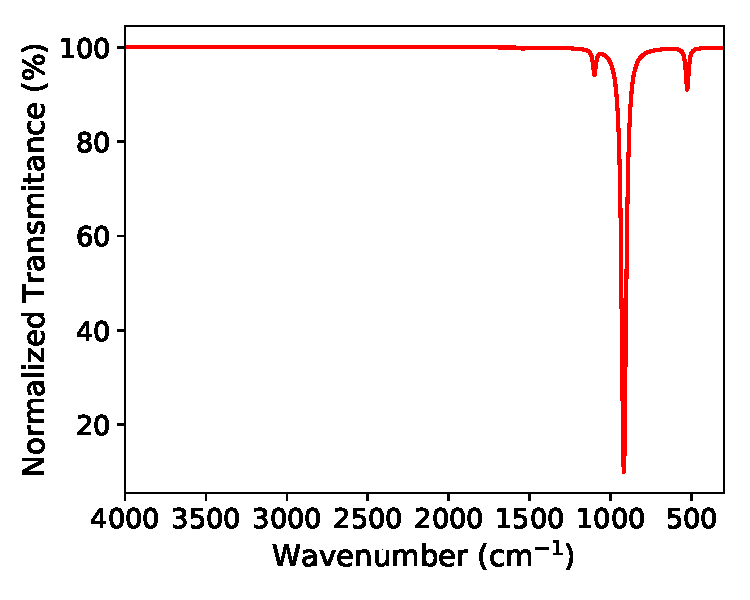
\includegraphics[width=.4\linewidth]{capitulos/fig/IR}}
		\subfloat{
			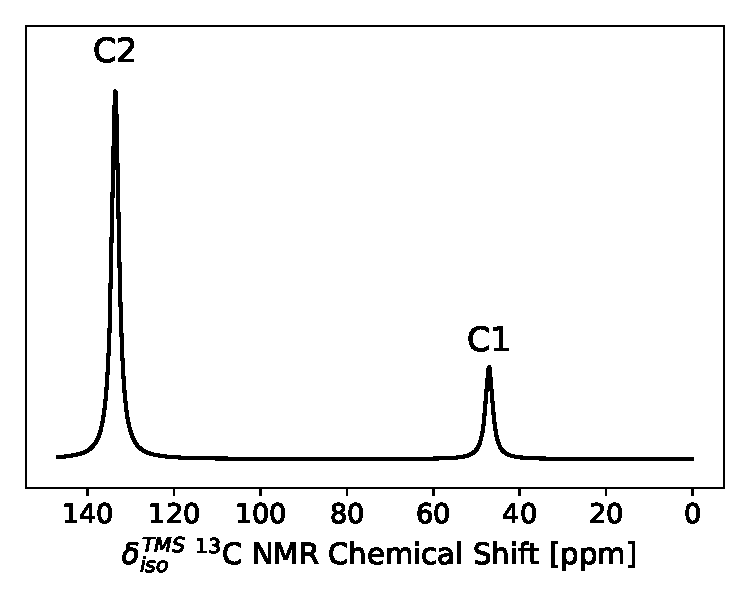
\includegraphics[width=.4\linewidth]{capitulos/fig/RMN}}\\
		\subfloat{
			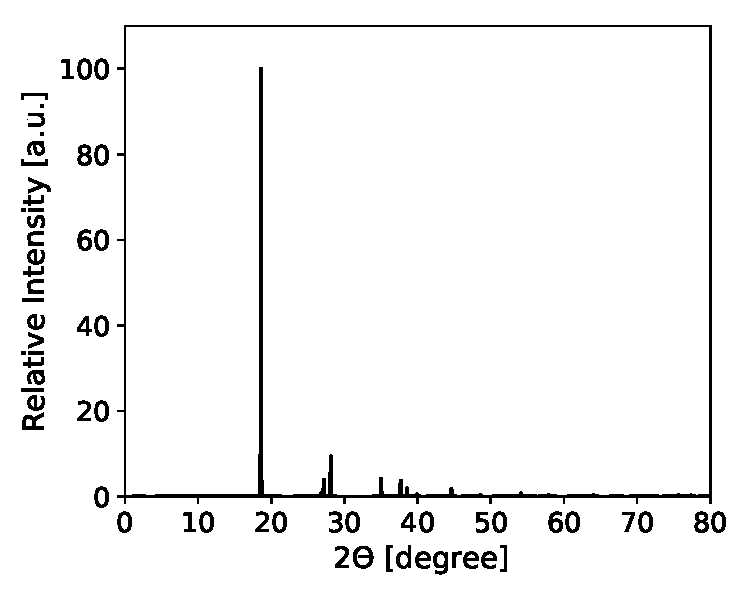
\includegraphics[width=.4\linewidth]{capitulos/fig/DRX}}
		\subfloat{
			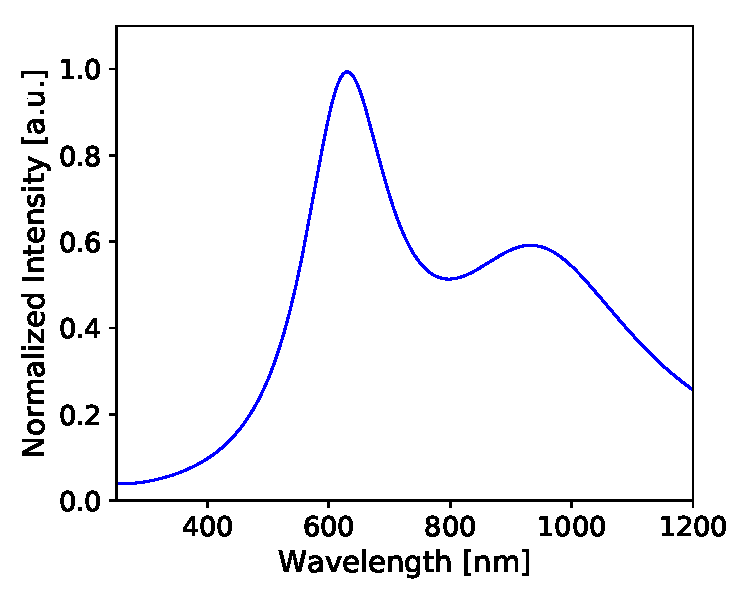
\includegraphics[width=.4\linewidth]{capitulos/fig/UV-VIS}}
		\caption{Gráficos dos espectros calculados de (a) FTIR (Lorentziana com 10 cm$^{-1}$ de largura); (b) deslocamentos químicos isotrópicos de \textsuperscript{13}C RMN (Lorentziana com 1 ppm de largura); (c) Difratograma de raios-X; (d) Espectro de absorção UV-VIS (Lorentziana com 0.02 Ry de largura)}
		\label{charac}
	\end{figure}

	Na \autoref{charac} são apresentados os espectros simulados de FTIR, \textsuperscript{13}C RMN, difração de raios-X e absorção no UV-VIS para o Spiro-Carbon, na esperança de que sejam úteis no auxílio da caracterização de possíveis candidatos. O espectro de FTIR (\autoref{charac}-\textbf{a}) apresenta um pico principal em 918 cm\textsuperscript{-1} devido ao modo vibracional com simetria E\textsubscript{u} e dois picos menores em 527 e 1100 cm\textsuperscript{-1} devido aos modos  E\textsubscript{u} and A\textsubscript{2u}, respectivamente. O espectro de \textsuperscript{13}C RMN, mostrado na \autoref{charac}-b, apresenta dois deslocamentos químicos diferentes: 47.0 ppm para o átomo C1 e 133.6 ppm para o átomo C2. O espectro de difração de raios-X, apresentado na \autoref{charac}-c, calculado para comprimento de onda de 1.54059 Å apresenta um pico principal em 18.5\textsuperscript{o} referente ao plano de Bragg (101) e picos menores em 29.8\textsuperscript{o} e 35.0\textsuperscript{o}, referentes aos planos (112) e (200), respectivamente.
	
	\subsection{Spiro-carbon como um material microporoso}
	
	\begin{figure}[ht]
		\centering
		\subfloat{
			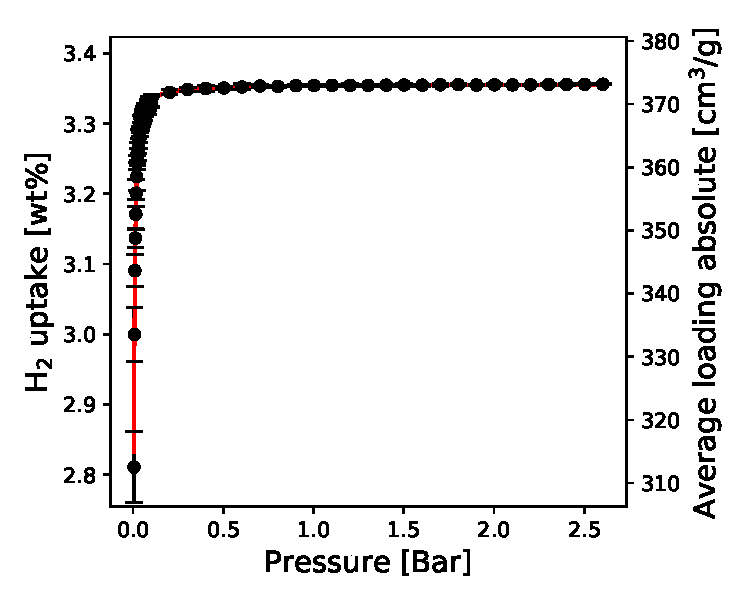
\includegraphics[width=.4\linewidth]{capitulos/fig/h2_h}}\\
		\subfloat{
			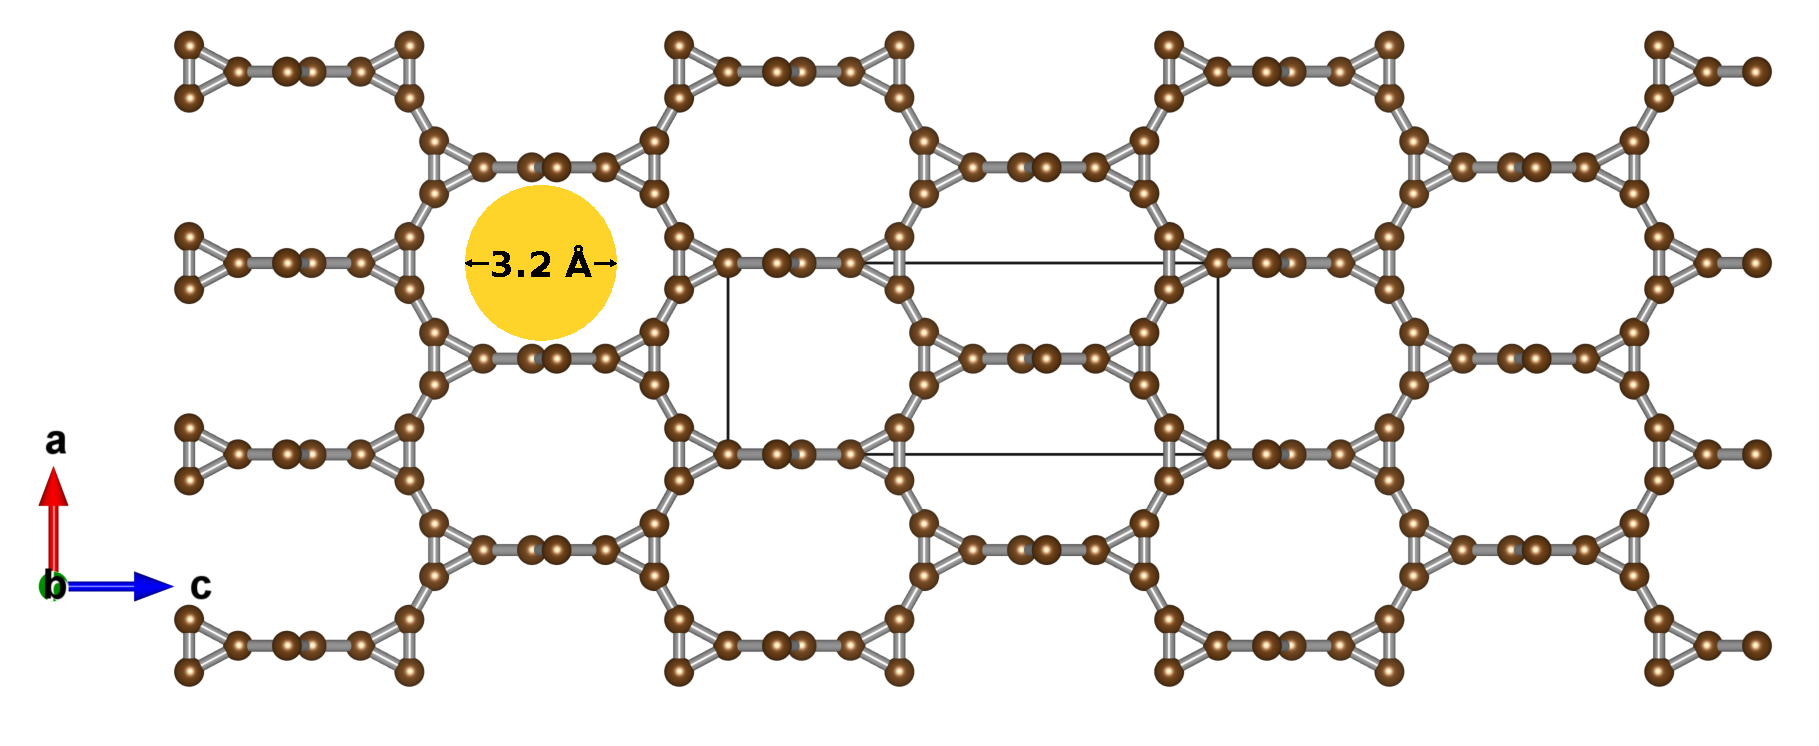
\includegraphics[width=0.8\linewidth]{capitulos/fig/pores.eps}}
		\caption{(a) Adsorção isotérmica de H\textsubscript{2}; (e) Representação da estrutura microporosa do Spiro-Carbon.}
		\label{charac_poros}
	\end{figure}

	Um aspecto que pode ser explorado nesse novo material proposto é sua estrutura porosa, representada na \autoref{charac_poros}-\textbf{b}. A máxima esfera que pode ser incluída dentro dos poros do Spiro-Carbon apresenta diâmetro de 3.21 Å. A área de superfície geometricamente acessível para essa estrutura é de 2296 m\textsuperscript{2}/g. Sendo assim, esse material poderia potencialmente ser um adsorvente seletivo para gases, particularmente aqueles compostos por moléculas pequenas, como H\textsubscript{2} por exemplo. Para avaliar a viabilidade desta aplicação cálculos Monte Carlo Grand-Canônicos foram executados a fim de obter a capacidade de adsorção de H\textsubscript{2}, N\textsubscript{2} e CO\textsubscript{2}. Na \autoref{charac_poros}-\textbf{a} pode-se observar uma isoterma de adsorção de H\textsubscript{2} do tipo I(a), típica de sólidos microporosos. \cite{thommes2015physisorption} 
	
	A capacidade adsortiva de H\textsubscript{2} à 77K em 1 bar (100 kPa) calculada foi de 373 cm\textsuperscript{3}/g, aproximadamente 3.35\% em peso. Esse valor é consideravelmente alto, o que inclui o Spiro-Carbon na classe de materiais microporosos com excepcional capacidade de adsorção de H\textsubscript{2}.  \cite{blankenship2017cigarette, wong2006exceptional} Cálculos similares para a adsorção de moléculas maiores, como N\textsubscript{2} e CO\textsubscript{2} revelaram que essas moléculas não caberiam dentro dos poros. Dessa forma, o Spiro-Carbon pode ser considerado um adsorvente seletivo e exclusivo para H\textsubscript{2}.
	
	\subsection{Conclusões}
	
		Nesta seção um novo alótropo de carbono nomeado Spiro-Carbon, que, na extensão de nosso conhecimento ainda não foi relatado na literatura, foi estudado por cálculos em nível DFT PBE-D3. Com base nos dados apresentados podemos concluir que esta estrutura é um mínimo na superfície de potencial, é mecanicamente estável e apresenta caráter eletrônico metálico peculiar. Ele também apresenta menor energia de formação que outras formas alotrópicas tridimensionais do carbono, como Y-, Y-II-, T-, e T-II-Carbon, e potencial aplicação como adsorvente seletivo para H$_2$.  
		
		Os resultados discutidos nesta seção resultaram na publicação do artigo:
		
		\begin{citacao}
			Oliveira, F.L., Capaz, R.B. and Esteves, P.M., \textit{Spiro-Carbon}: A metallic carbon allotrope predicted from first principles calculations. \textbf{Chem. Phys. Chem.}, v.21, n.1, p.59-64, 2020.
		\end{citacao}
		
\section{ABF-Carbon}
		
		Tomando com base o motivo estrutural explorado no alótropo de carbono da seção anterior, o motivo \textbf{\textit{spiro}}, podemos conceber uma miríade de outras estruturas. Poderíamos, por exemplo, utilizar a estratégia de inserir unidades de acetileno entre as unidades spiro, formando estruturas conjugadas com poros progressivamente maiores como explorado em \cite{costa2018n}. Por outro lado, é possível conectar o motivo estrutural diretamente a átomos de carbono \textit{sp\textsuperscript{3}}, formando estruturas porosas semelhantes ao Spiro-Carbon, porém sem a conjugação entre as ligações duplas, gerando um potencial alótropo de carbono 3D semi-condutor. Essa estrutura hipotética será explorada ao longo dessa próxima seção.
	
	\subsection{Estrutura}
	
				
		\begin{figure}[ht!]
			\centering
			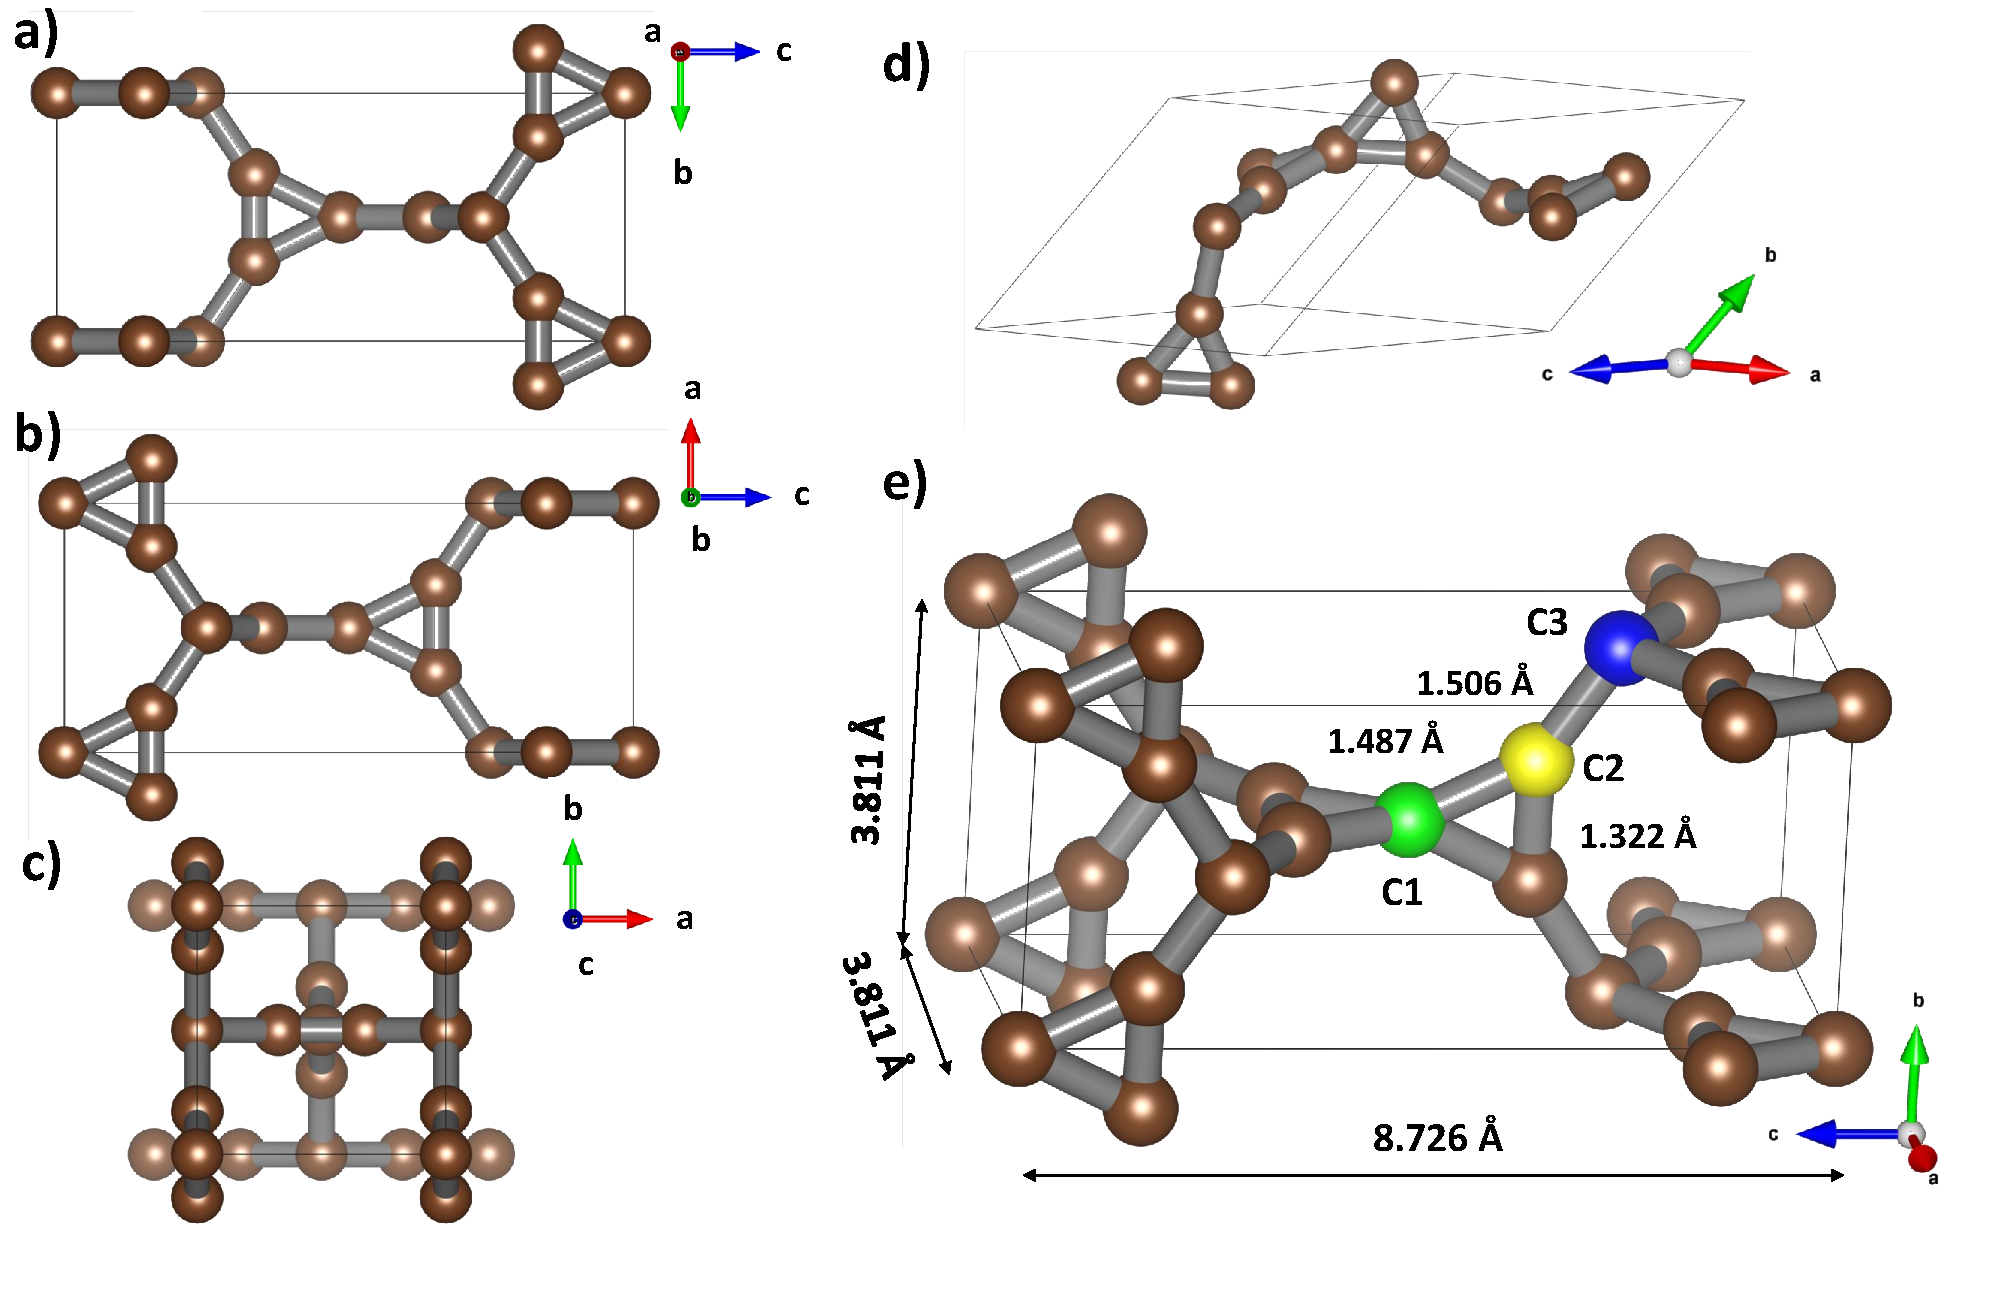
\includegraphics[width=.9\linewidth]{capitulos/fig/results2/structure}
			\caption{Representação da célula unitária do ABF-Spiro vista na direção dos vetores a) \textbf{a}, b) \textbf{b}, c) \textbf{c}, d) representação de célula primitiva e e). Representação da estrutura atômica da célula unitária tetragonal para o ABF-Carbon, com os átomos não equivalentes destacados em cores diferentes.}
			\label{structure_homospiro}
		\end{figure}	
	
		Essa estrutura idealizada, que pode representada por uma rede 3D do tipo \textbf{abf} \footnote{http://rcsr.anu.edu.au/nets/abf\#} e por isso será nomeada como ABF-Carbon, apresenta 6 átomos em uma célula unitária primitiva tetragonal de corpo centrado, com grupo espacial $I\bar{4}m2$ (\#119) e grupo pontual $D_{2d}^{11}$. A geometria de equilíbrio obtida a partir da otimização completa da estrutura apresenta parâmetros de célula \textit{a} = \textit{b} = 3.811 Å, \textit{c} = 8.726 Å e $\alpha$ = $\beta$ = $\gamma$ = 90$^\circ$, apresentando densidade de 1.89 g/cm$^3$. A célula unitária primitiva e convencional resultante é apresentada na \autoref{structure_homospiro}.

		
		Baseado na simetria do grupo espacial desta estrutura os três átomos não equivalentes ocupam os sítios de Wyckoff 8i, 2a e 2d, como representado na \autoref{structure_homospiro}-e). O átomo \textbf{C1} (verde) ocupa o sítio 8i e apresenta coordenadas fracionárias (0.00000, 0.00000, 0.00000), \textbf{C2} (amarelo) ocupa o sítio 2a e apresenta coordenadas (0.82651, 0.00000, 0.15266) e \textbf{C3} (azul) ocupa o sítio 2d apresentando coordenadas (0.00000, 0.50000, 0.75000). Baseado na estrutura otimizada é possível distinguir três diferentes tipos de ligação: \textit{i)} As ligações do átomo $sp^3$ da unidade \textit{spiro} com seus vizinhos (C1-C2) com comprimento iguais de 1.487 Å; \textit{ii)} as ligações entre os átomos \textbf{C2} (C2=C2), com comprimento de 1.322 Å, fechando o anel de 3 membros e formando a unidade spiro; \textit{iii)} as ligações das unidades \textit{spiro} com o átomo de carbono $sp^3$ (\textbf{C3}), com comprimento de 1.506 \AA, comprimento típico de ligação simples entre átomos de carbono.
		
		Os ângulos internos da unidade \textit{spiro} são de 52.8$^\circ$ (C2-C1-C2) e 63.6$^\circ$ (C1-C2-C2), valores iguais aos apresentados pelo análogo molecular spiropentadieno. Os ângulos das ligações do átomo de carbono \textbf{C3} apresentam um leve desvio do padrão para um tetraedro perfeito, de 109.5$^\circ$, apresentando valores de 111.4$^\circ$ e 108.5$^\circ$.     
		
		É possível observar que nessa estrutura que os comprimentos e ângulos das ligações na unidade \textit{spiro} se assemelham muito mais ao seu análogo molecular, o spiropentadieno, do que na estrutura do Spiro-Carbon. Isso se dá pelo fato de que, nessa estrutura, as unidades \textit{spiro} estão ligadas diretamente a átomos de carbono $sp^3$, o que impede que ocorra a conjugação entre as ligações duplas e fazendo que as ocorra uma localização maior das ligações duplas e simples. Isso nos permite antecipar que essa estrutura apresentará um caráter semi-condutor com \textit{band gap} relativamente grande, devido à dificuldade de interação entre os orbitais $\pi$. 
		
	\subsection{Estabilidade Relativa e Propriedades Mecânicas}
	
		Para investigar a estabilidade relativa desta estrutura, foi calculada a dispersão de fônons ao longo de um caminho entre pontos de alta simetria na primeira zona de Brillouin \cite{bradley2010mathematical}. Como pode ser observado na \autoref{ph_DOS-2}-\textbf{a)} não há a presença de nenhuma frequência imaginária, indicando que a estrutura do ABF-Carbon corresponde a um mínimo na superfície de potencial. 
	
		\begin{figure}[ht]
			\centering
			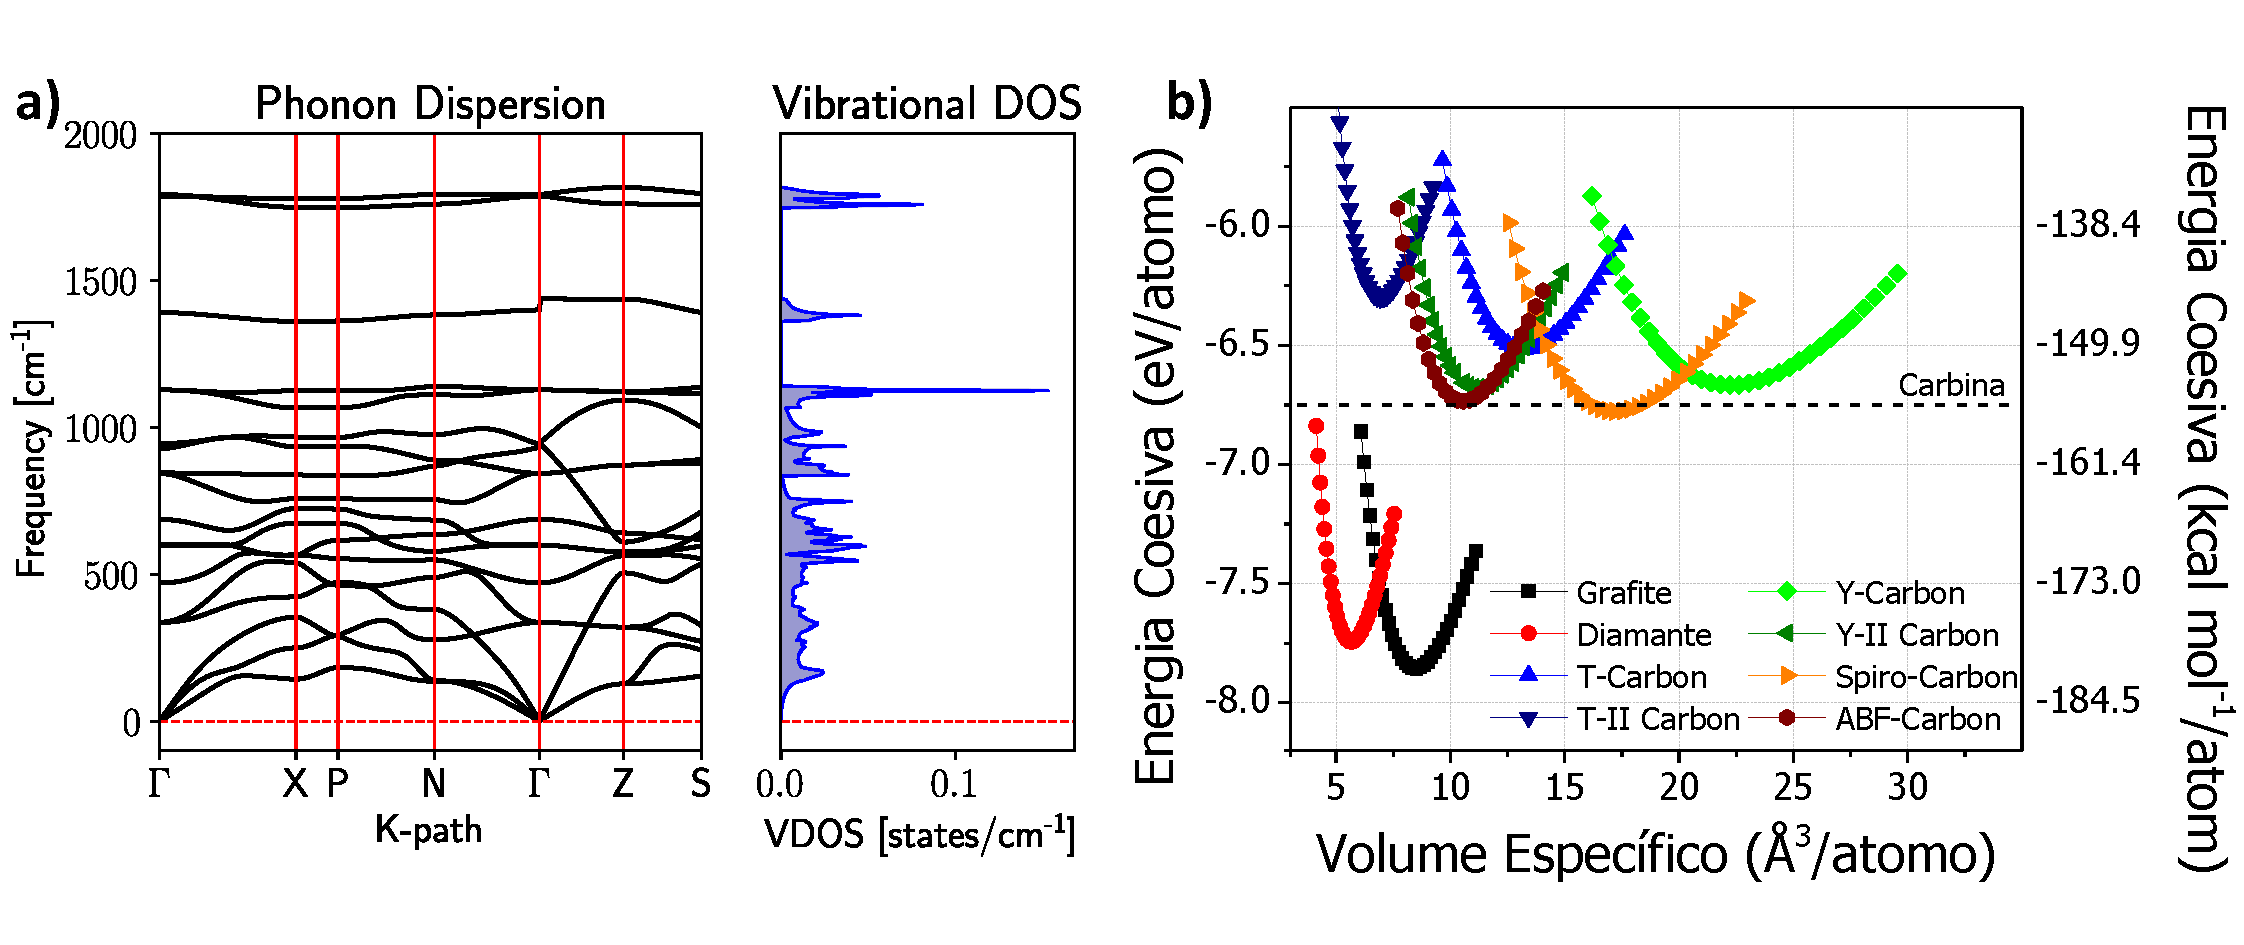
\includegraphics[width=1\linewidth]{capitulos/fig/results2/cohesive_abf-carbon}
			\caption{Gráfico da dispersão de fônons ao longo de alguns pontos de alta simetria na primeira zona de Brillouin e a correspondente densidade de estados vibracionais (VDOS) para o ABF-Carbon.}
			\label{ph_DOS-2}
		\end{figure}

		Para avaliar a estabilidade termodinâmica relativa do ABF-Carbon, a \autoref{ph_DOS-2}-\textbf{b)} mostra a variação da energia coesiva em função do volume (ambos por átomo) para diferentes alótropos de carbono. Como esperado, a curva $E_c(V)$ para o ABF-Carbon apresenta claramente um mínimo correspondente ao estado meta-estável desta estrutura. Assim como o Spiro-Carbon, esta estrutura se mostrou mais estável do que outros alótropos de carbono tridimensionais  como  1-diamantino/Y-Carbon \cite{costa2018n,li2014modulated} por aproximadamente 1.55 kcal/mol (0.07 eV) por átomo e o T-Carbon \cite{sheng2011t} por aproximadamente 5.1 kcal/mol (0.22 eV), como mostrado na \autoref{energy-abf}. 
		
		Curiosamente o ABF-Carbon apresentou energia coesiva cerca de 1.0 kcal/mol (0.05 eV) menor do que o Spiro-Carbon. Em geral, é esperado que uma estrutura que apresente mais átomos de carbono com hibridização $sp^3$ apresente maior estabilidade, entretanto, o ABF-Carbon mesmo apresentando uma razão de átomos $sp^2$/$sp^3$ de 2/1, valor menor do que o apresentado pelo Spiro-Carbon de 4/1, apresenta menor energia de formação. Este fenômeno é bastante incomum, e pode ter uma relação direta com o fato de o grafite possuir energia coesiva maior do que o diamante. Talvez a deslocalização gerada pela formação de ligações $\pi$ conjugadas, como acontece no grafite e no Spiro-Carbon, seja um fator estabilizante maior do que a sobreposição frontal dos orbitais gerada pela formação das ligações $\sigma$ em estruturas como a do diamante e do ABF-Carbon. Esse fenômeno ainda não apresenta uma resposta conclusiva na literatura, e pesquisas mais aprofundadas devem ser feitas para tentar explicar esse resultado contra-intuitivo. 
		
		\begin{table*}[ht]
			\centering
			\renewcommand{\arraystretch}{1.1}
			\caption{Módulo das energias relativa e coesiva por átomo para o ABF-Carbon comparado com diferentes alótropos de carbono.}
			\label{energy-abf}
			\begin{tabular}{lcccc}
				\hline
				\hline
				\multicolumn{1}{c}{\multirow{2}{*}{Estrutura}} & \multicolumn{2}{c}{Energia Relativa} & \multicolumn{2}{c}{Energia Coesiva}                             \\ \cline{2-5} 
				\multicolumn{1}{c}{}                           & \multicolumn{1}{l}{eV/átomo} & \multicolumn{1}{l}{kcal/mol/átomo} & \multicolumn{1}{l}{eV/átomo} & \multicolumn{1}{l}{kcal/mol/átomo} \\ \hline
				Grafite      & 0.000  & 0.000  & 7.856  & 181.16  \\
				Diamante     & 0.112  & 2.57   & 7.744  & 178.59  \\
				Spiro-Carbon & 1.079  & 24.88  & 6.777  & 156.29  \\
				Carbina      & 1.106  & 25.50  & 6.750  & 155.67  \\
				ABF-Carbon   & 1.121  & 25.86  & 6.735  & 155.30  \\
				Y Carbon     & 1.189  & 27.41  & 6.667  & 153.75  \\
				Y-II Carbon  & 1.177  & 27.15  & 6.679  & 154.01  \\
				T Carbon     & 1.342  & 30.94  & 6.514  & 150.22  \\
				T-II Carbon  & 1.554  & 35.84  & 6.302  & 145.32  \\ \hline \hline
			\end{tabular}
		\end{table*}
		
		
		Avaliando as seis constantes elásticas ($\textbf{C}_{ij}$ em GPa) calculadas, apresentadas na \autoref{elastic_ABF}, é fácil ver que as condições necessárias e suficientes que devem ser satisfeitas, baseadas nos critérios de estabilidade de Born \cite{born1940stability}, para garantir a estabilidade mecânica para uma rede tetragonal são satisfeitos pelo ABF-Carbon, indicando que essa nova estrutura proposta é mecanicamente estável. 
		
		\begin{table}[ht]
			\centering
			\renewcommand{\arraystretch}{1.1}
			\caption{Constantes elásticas ($\textbf{C}_{ij}$), módulo Bulk (\textbf{B}), shear (\textbf{G}) e Young (\textbf{E}) (em GPa), razão de Poisson ($\nu$) e dureza de Vicker ($H_v$) calculados para o Diamante, Spiro-Carbon e ABF-Carbon}
			\label{elastic_ABF}
			\begin{tabular}{lccc}
				\hline \hline
				& Diamante & Spiro-Carbon & ABF-Carbon \\\hline
				\textbf{C\textsubscript{11}} & 1106.43   & 277.76   & 481.72  \\
				\textbf{C\textsubscript{33}} & 1106.43   & 308.54   & 560.51  \\
				\textbf{C\textsubscript{44}} &  591.34   & 75.04    & 120.03  \\
				\textbf{C\textsubscript{66}} &  591.34   & 3.61     &  38.09  \\
				\textbf{C\textsubscript{12}} &  153.08   & 3.36     &  10.04  \\
				\textbf{C\textsubscript{13}} &  153.08   & 68.88    &  90.13  \\
				\textbf{B}                   &  470.86   & 123.73   & 209.37  \\
				\textbf{G}                   &  542.45   & 47.79    & 120.30  \\
				\textbf{E}                   & 1175.83   & 121.98   & 301.40  \\
				\textbf{$\nu$}               &   0.084   & 0.276    & 0.253   \\
				\textbf{$H_v$}               &   90.87   & 4.37    & 14.23   \\
				\hline \hline
			\end{tabular}
			\noindent
		\end{table}
		
		
		
		\begin{figure*}[!ht]
			\centering
			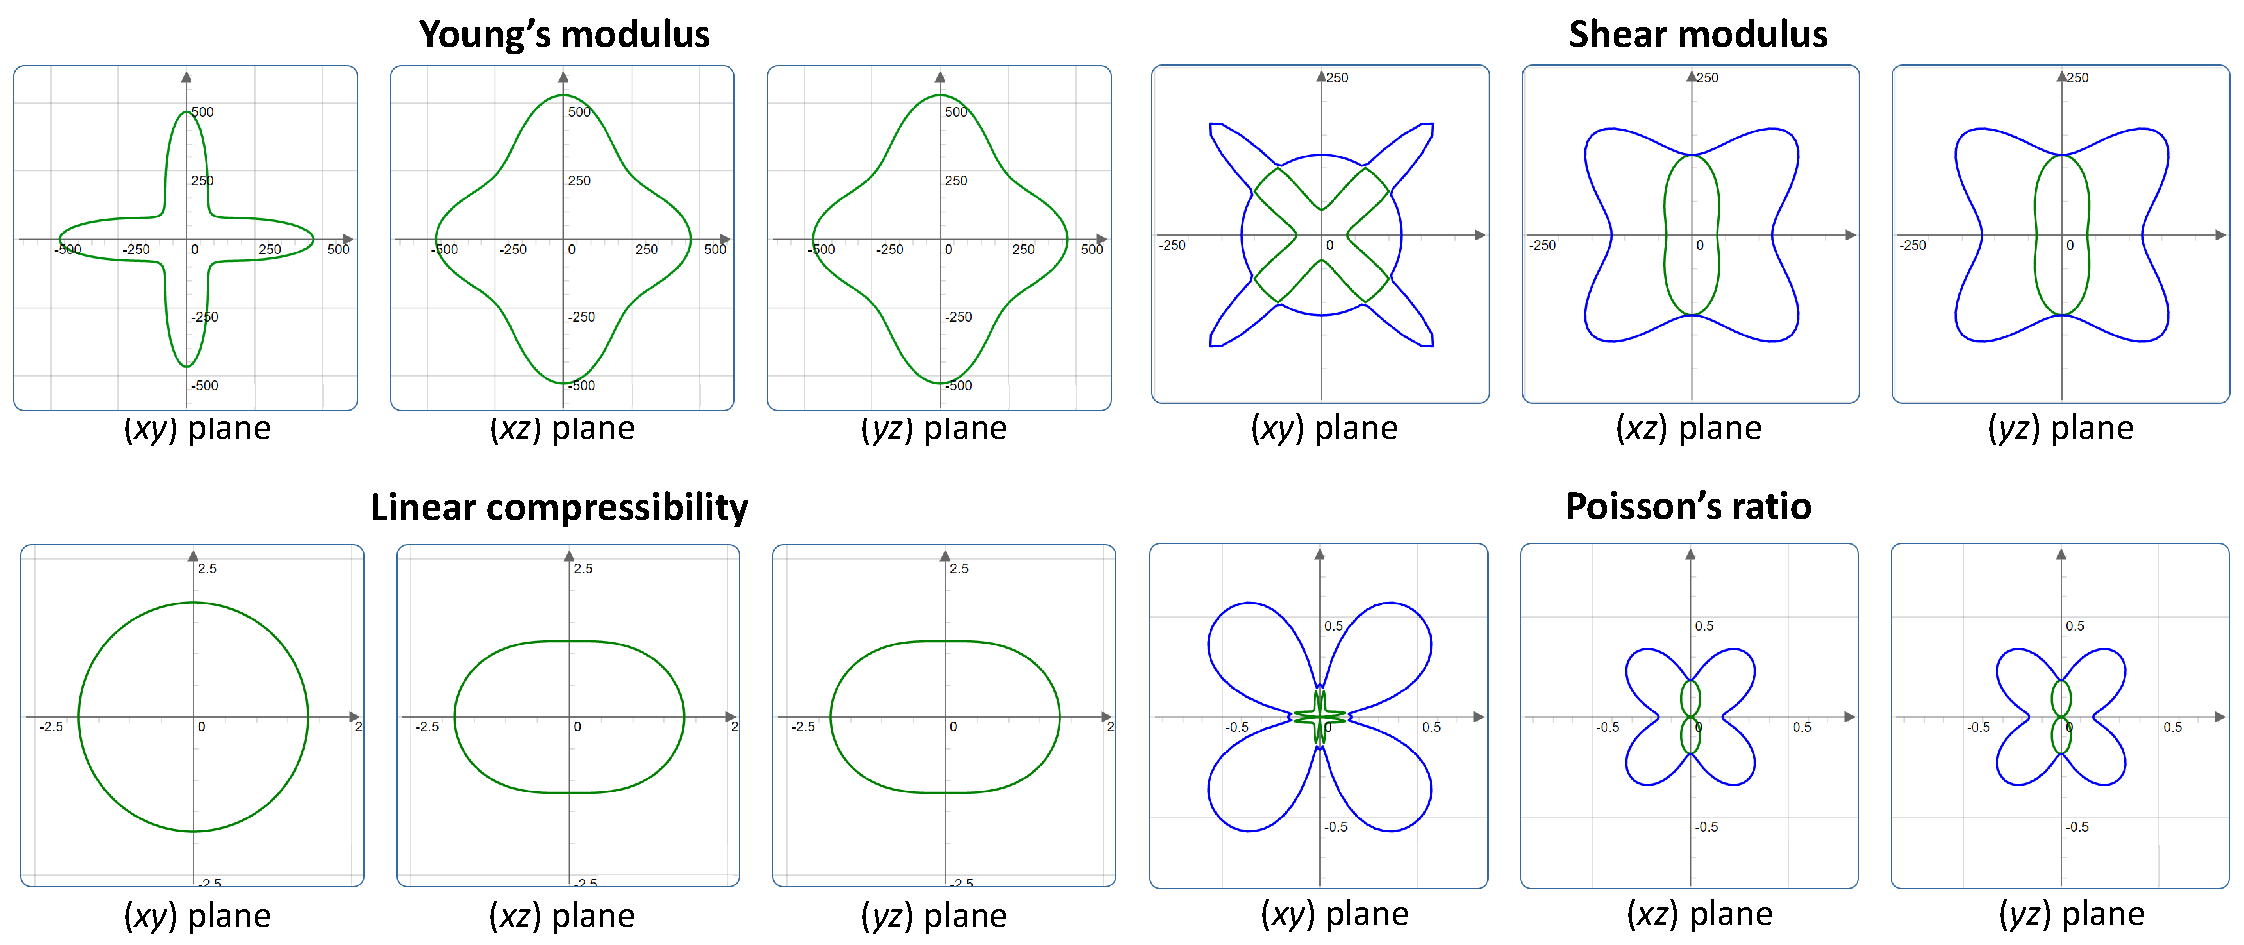
\includegraphics[width=1\linewidth]{capitulos/fig/results2/elastic_abf}
			\caption{Dependência espacial do (a) módulo de Young; (b) compressibilidade linear; (c) módulo Shear e (d) razão de Poisson para o ABF-Carbon.}
			\label{plot_elastic_ABF}
		\end{figure*}
		
		A \autoref{plot_elastic_ABF} mostra os gráficos da dependência espacial nos planos \textbf{xy}, \textbf{xz} e \textbf{yz} para os módulos de Young (\textbf{E}) e shear (\textbf{G}), compressibilidade linear  ($\beta$) e razão de Poisson ($\nu$), calculadas a partir das constantes elásticas apresentadas na \autoref{elastic_ABF}. É possível notar uma anisotropia do módulo de Young e módulo shear semelhante à apresentada pelo Spiro-Carbon, porém com menor intensidade. Esse resultado pode ser associado com a presença do átomo de carbono $sp^3$ conectando as unidade spiro na formação da estrutura estendida, conferindo maior rigidez e menor anisotropia a esse material. De fato, a anisotropia do módulo de Young é de A\textsubscript{E} = 4.03 e do módulo de cisalhamento é de A\textsubscript{G} = 5.55, valores muito menores que o para o Spiro-Carbon que são de 19.58 e 29.98, respectivamente.
			
		Utilizando o modelo empírico de \citeauthor{chen2011modeling} para o cálculo  da dureza de Vicker, o valor obtido para o ABF-Carbon é de 14.23 GPa (1452 HV). Esse valor é 3.25 vezes maior do que o apresentado pelo Spiro-Carbon, confiando que a adição dos átomos de carbono sp$^3$ na estrutura aumentam sua rigidez e dureza.
		%1 HV = 0.009807 GPa
		
	\subsection{Propriedades Eletrônicas}
		
		A estrutura do ABF-Carbon, ao contrário do Spiro-Carbon, apresenta ligações duplas localizadas nas unidades \textit{spiro} sem a possibilidade de conjugação, fazendo com que esse material possa apresentar um caráter semi-condutor. O \textit{gap} HOMO-LUMO calculado para a molécula do spiropentadieno é de 3.92 eV e 5.22 eV quando calculado como os funcionais PBE e HSE, respectivamente.\footnote{Ver Apêndice \autoref{chap:spiropentadiene} para mais detalhes} O diagrama de bandas calculado em nível PBE, apresentado na \autoref{band_ABF}, confirma o caráter semi-condutor com \textit{band gap} direto da estrutura. Além disso, é possível observar que a densidade de estados próxima ao nível de Fermi é formada unicamente pelos orbitais $2p$ ($2p_x$, $2p_y$ e $2p_z$). O \textit{band gap} direto calculado nesse nível é de 1.35 eV e 2.39 eV com o funcional HSE, indicando que essa estrutura apresenta um grande potencial para aplicações em optoeletrônica e fotocatálise.
		
		
		\begin{figure}[!ht]
			\centering
			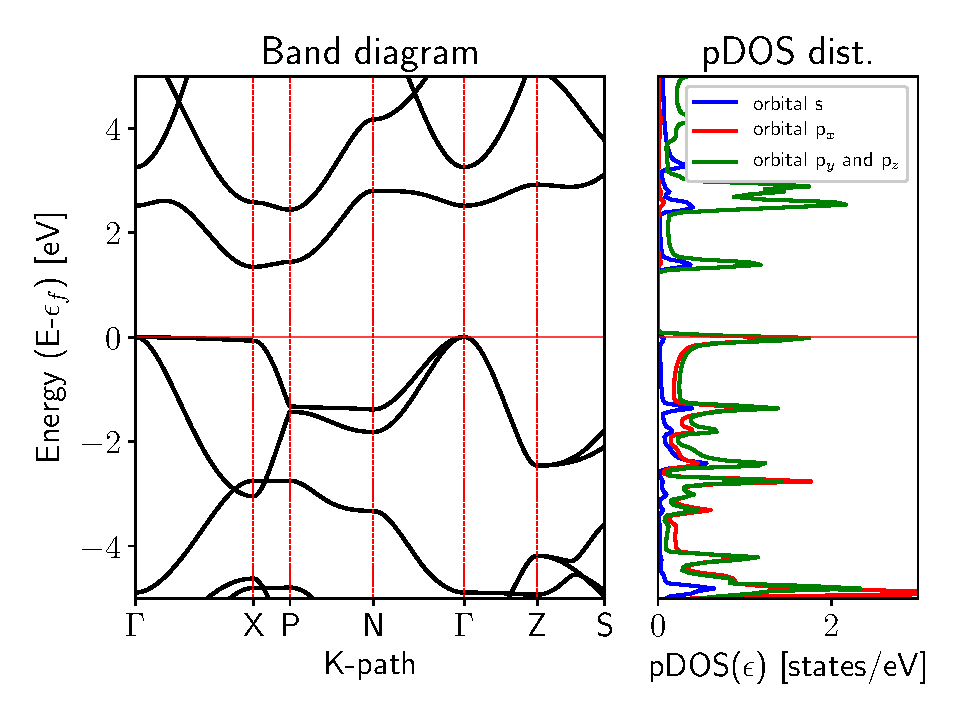
\includegraphics[width=.7\linewidth]{capitulos/fig/results2/band_structure}
			\caption{Dispersão de energia das bandas ao longo dos principais pontos de alta simetria na primeira zona de Brillouin (direita) e densidade de estados projetada nos orbitais (esquerda) para o ABF-Carbon. A energia de Fermi ($\epsilon_f$) foi ajustada para 0.}
			\label{band_ABF}
		\end{figure}
		
	\subsection{Caracterização}
		
		Na \autoref{carac_abf} são apresentados os espectros simulados de FTIR, \textsuperscript{13}C RMN e difração de raios-x e espectro de absorção no UV-VIS para o ABF-Carbon, na esperança de que sejam úteis no auxílio da caracterização de possíveis candidatos. O espectro de FTIR (\autoref{carac_abf}-\textbf{a}) apresenta um pico principal em 1391 cm\textsuperscript{-1} devido ao modo vibracional com simetria B\textsubscript{2} e um pico  em 927 cm\textsuperscript{-1} devido a outro modo B\textsubscript{2}. O espectro de \textsuperscript{13}C RMN, mostrado na \autoref{carac_abf}-\textbf{b}, apresenta três deslocamentos químicos diferentes: 128.5 ppm para o átomo C1, 44.2 ppm para o átomo C2 e 39.2 para o átomo C3. O espectro de difração de raios-X, apresentado na \autoref{carac_abf}-\textbf{c}, calculado para comprimento de onda de 1.54059 Å apresenta um pico principal em 25.5\textsuperscript{o} referente ao plano de Bragg (101) e picos menores em 20.3\textsuperscript{o} e 33.2\textsuperscript{o}, referentes aos planos (002) e (110), respectivamente. O espectro de absorção na região do UV-VIS apresenta bandas em 280, 320, 480 e 960 nm, indicando grande potencial para aplicações que dependam de absorção de luz em regiões no espectro visível e próximas. Essa estrutura não apresentam poros com tamanho suficiente para ser acessível a nenhum átomo ou molécula. 
	
		\begin{figure}[!ht]
			\centering
			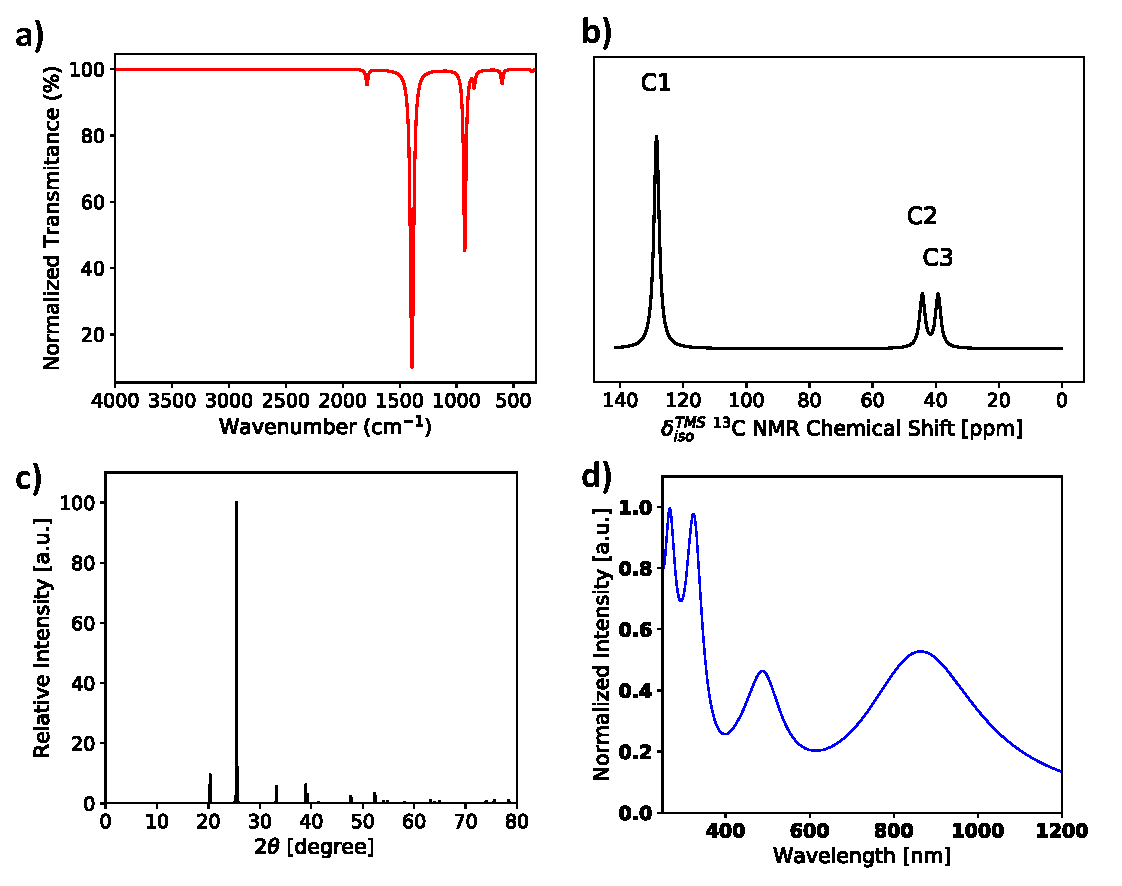
\includegraphics[width=1\linewidth]{capitulos/fig/results2/carac_ABF}
			\caption{Gráficos dos espectros calculados de (a) FTIR (Lorentziana com 10 cm$^{-1}$ de largura); (b) deslocamentos químicos isotrópicos de \textsuperscript{13}C RMN (Lorentziana com 1 ppm de largura); (c) Difratograma de raios-X; (d) Espectro de absorção no UV-VIS (Lorentziana com 0.02 Ry de largura).}
			\label{carac_abf}
		\end{figure}

	\subsection{Conclusões}
	
		Nesta seção foi apresentado um novo alótropo de carbono, denominado ABF-Carbon, formado pela conexão de unidades \textit{spiro} por átomos de carbono sp\textsuperscript{3}. Com base nos resultados apresentados é possível concluir que essa nova estrutura é estável, pois não apresenta frequências negativas na dispersão de fônons e sua matriz elástica satisfaz os critérios de estabilidade de Born. Diferentemente do Spiro-Carbon, essa estrutura apresenta um caráter semicondutor, com \textit{band gap} de 2.4 eV. Além disso, ela apresenta menor energia de formação que outras estruturas alotrópicas tridimensionais, encorajando possíveis tentativas de síntese.

\chapter{Gerando novos alótropos}
\label{alotropos_carbina}
	
	Na \autoref{sec:spiro} deste trabalho foi apresentado a estrutura do Spiro-Carbon e um dos aspectos mais marcantes é sua semelhança com cadeias de \textit{trans-cisoide}-(poli)acetileno conectadas por átomos de carbono $sp^3$, a origem de seu caráter metálico. Apesar de não ser um conceito prático, afinal polimerizar cadeias de (poli)acetileno para formar a estrutura cristalina do Spiro-Carbon pode ser um desafio sintético insuperável, utilizar uma molécula, ou motivo estrutural derivado de uma, como bloco de construção pode ser uma estratégia promissora para a idealização de novos alótropos de carbono.
	
	De fato, alguns trabalhos recentes na literatura mostram que utilizar alótropos já existentes como ponto de partida para novas estruturas pode ser uma ótima estratégia. \citeauthor{hu2013compressed} em \citeyear{hu2013compressed} mostrou que nanotubos de carbono comprimidos podem reorganizar suas ligações e formar novas estruturas. \citeauthor{fedik2020can} em \citeyear{fedik2020can} mostrou que o cyclo[18]carbon pode ser entrelaçado, como anéis em uma corrente, para formar catenanos de carbono. 
			
	\begin{figure}[!ht]
		\centering
		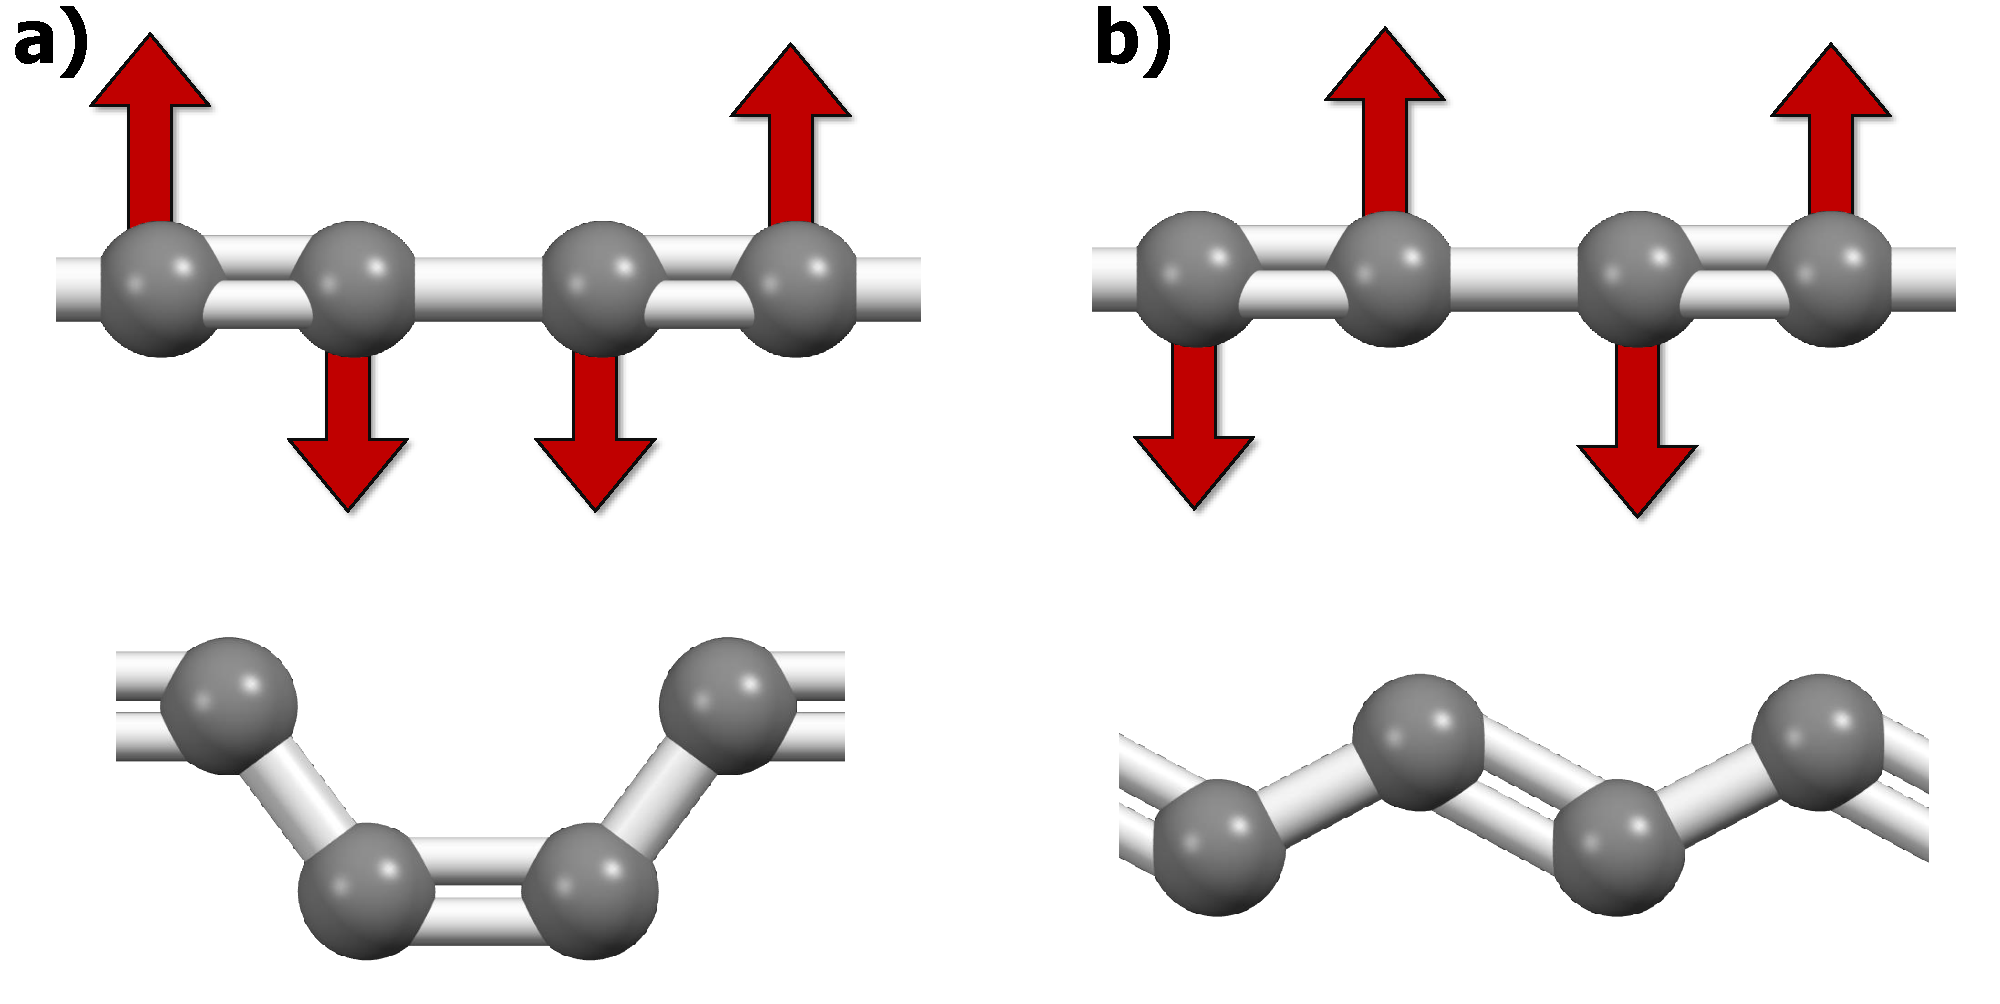
\includegraphics[width=.7\linewidth]{capitulos/fig/results3/carbina}
		\caption{Possíveis distorções da cadeia do carbino.}
		\label{carbina}
	\end{figure}

	Se olharmos para os modos normais de vibração do carbino, como apresentado na \autoref{carbina}, é possível perceber que dependendo de como esse modos se acoplam podem ser geradas duas formas muito parecidas com as diferentes configurações da cadeia de (poli)acetileno: um carbino em forma \textit{armchair} \textbf{(a)}, semelhante ao \textit{cis}-(poli)acetileno, e uma em forma \textit{zigue-zague} \textbf{(b)}, semelhante ao \textit{trans}-(poli)acetileno.
	
	Dessa forma, é possível pensar na formação de alótropos de carbono como o grafeno, ou até mesmo o Spiro-Carbon, a partir de cadeias do carbino distorcidas na direção de um de seus modos normais de vibração. Se a cadeia for distorcida na forma \textit{zigue-zague} e forem aproximadas de maneira paralela poderia ocorrer a quebra de uma ligação $\pi$ e consequente formação de ligações entre as cadeias, gerando assim a estrutura do grafeno. Por outro lado, se as cadeias fossem distorcidas na forma \textit{armchair} e fossem aproximadas de um átomo de carbono de maneira perpendicular, poderia ocorrer a formação da estrutura do Spiro-Carbon. É importante ressaltar que esse método não é uma proposta de mecanismo de síntese, mas sim puramente um exercício mental para desenvolver uma lógica de construção de novas estruturas. 
	
	A partir dessa metodologia, o grafeno e o Spiro-Carbon não são as únicas estruturas que podem ser geradas. Podemos conectar as cadeias distorcidas na forma zigue-zague não paralelamente, como é feito para gerar o grafeno, mas sim perpendicularmente e obter a estrutura proposta por \citeauthor{hoffmann1983hypothetical} em \citeyear{hoffmann1983hypothetical}. Podemos conectar as cadeias do carbino não por apenas um átomo, mas por dois ou mais átomos de carbono gerando assim uma miríade de estruturas, como representado na \autoref{alotropos}. 
	
	\begin{figure}[!ht]
		\centering
		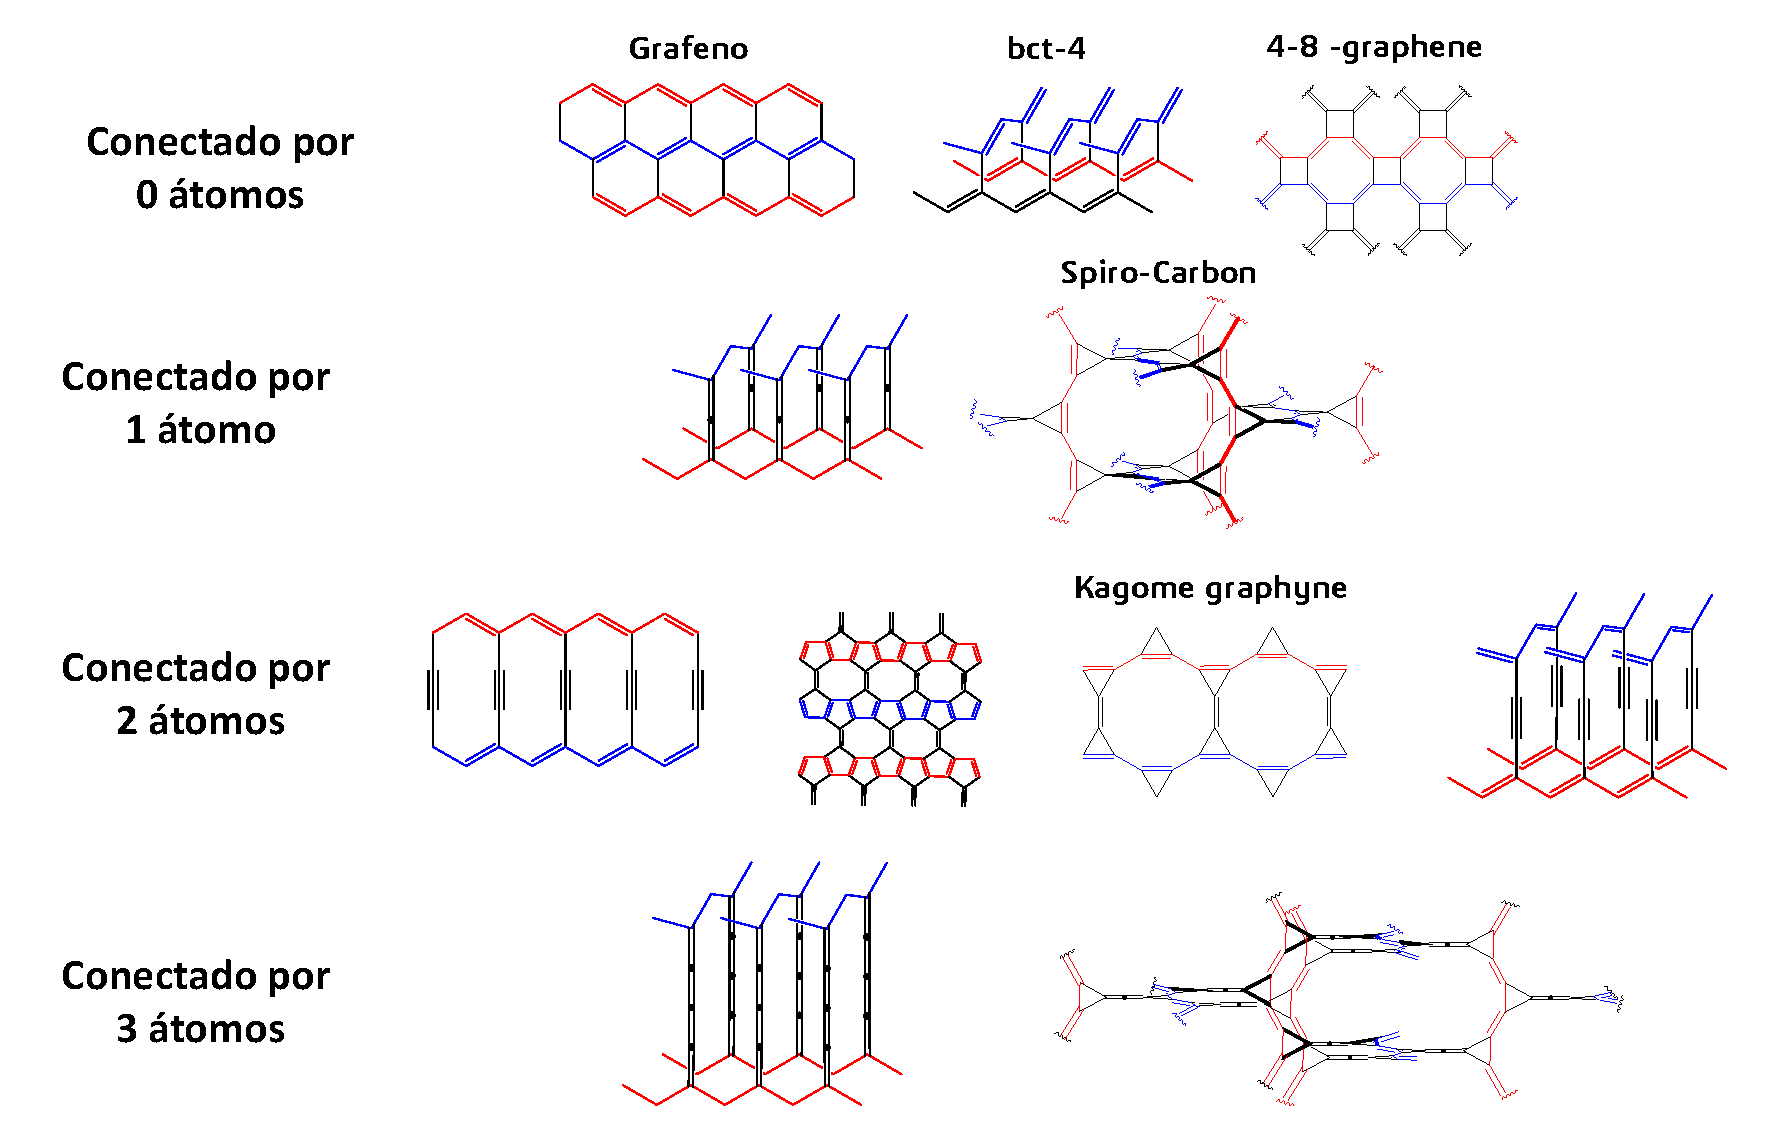
\includegraphics[width=1.\linewidth]{capitulos/fig/results3/alotropos}
		\caption{Diferentes alótropos que podem ser gerados a partir das diferentes formas de conectar o carbino.}
		\label{alotropos}
	\end{figure}

	\section{Conectando as cadeias diretamente}
		
		Seguindo a lógica de construção proposta, podemos gerar três estruturas diferentes conectando as cadeias diretamente. Utilizando a cadeia de carbino distorcida na forma \textit{zigue-zague} pode-se gerar a estrutura do grafeno (\autoref{0atomos}-\textbf{a}), se conectadas de maneira paralela, e a do bct-4 (\autoref{0atomos}-\textbf{b}), explorada por \citeauthor{hoffmann1983hypothetical}, se conectadas de maneira perpendicular. Utilizando a cadeia deformada na forma \textit{armchair} conectada diretamente de maneira paralela pode-se obter a estrutura (4,8)-carbon (\autoref{0atomos}-\textbf{c}), explorada por \citeauthor{nisar2012semiconducting}. Não é possível formar uma estrutura estável com a forma \textit{armchair} conectada perpendicularmente, pois dessa forma a distância entre dois átomos de cadeias adjacentes seria próxima do comprimento de uma ligação simples ($\approx$1.5 Å). 
		
		A \autoref{0atomos} apresenta os cálculos do diagrama de bandas e dispersão de fônons para as três possíveis estruturas. É possível observar que nos três casos elas apresentam interseção entre as bandas de valência e condução, mostrando o caráter metálico já conhecido para essas estruturas. Uma característica que não é apresentada na literatura é a dispersão de fônons para o bct-4 (\autoref{0atomos}-\textbf{b}) e o (4,8)-carbon (\autoref{0atomos}-\textbf{c}). Os resultados para ambas as estruturas mostram uma grande incidência de modos vibracionais imaginários, indicando que nenhuma das estruturas é estável. De fato, no artigo original do bct-4 carbon os autores comentam que essa estrutura poderia apresentar uma espécie de "tensão $\pi$", devido à proximidade entre os orbitais $\pi$ na vizinhança de cada cadeia. Esse fator pode ser responsável pelas frequências vibracionais imaginárias apresentadas em \textbf{N}.
		
		\begin{figure}[!ht]
			\centering
			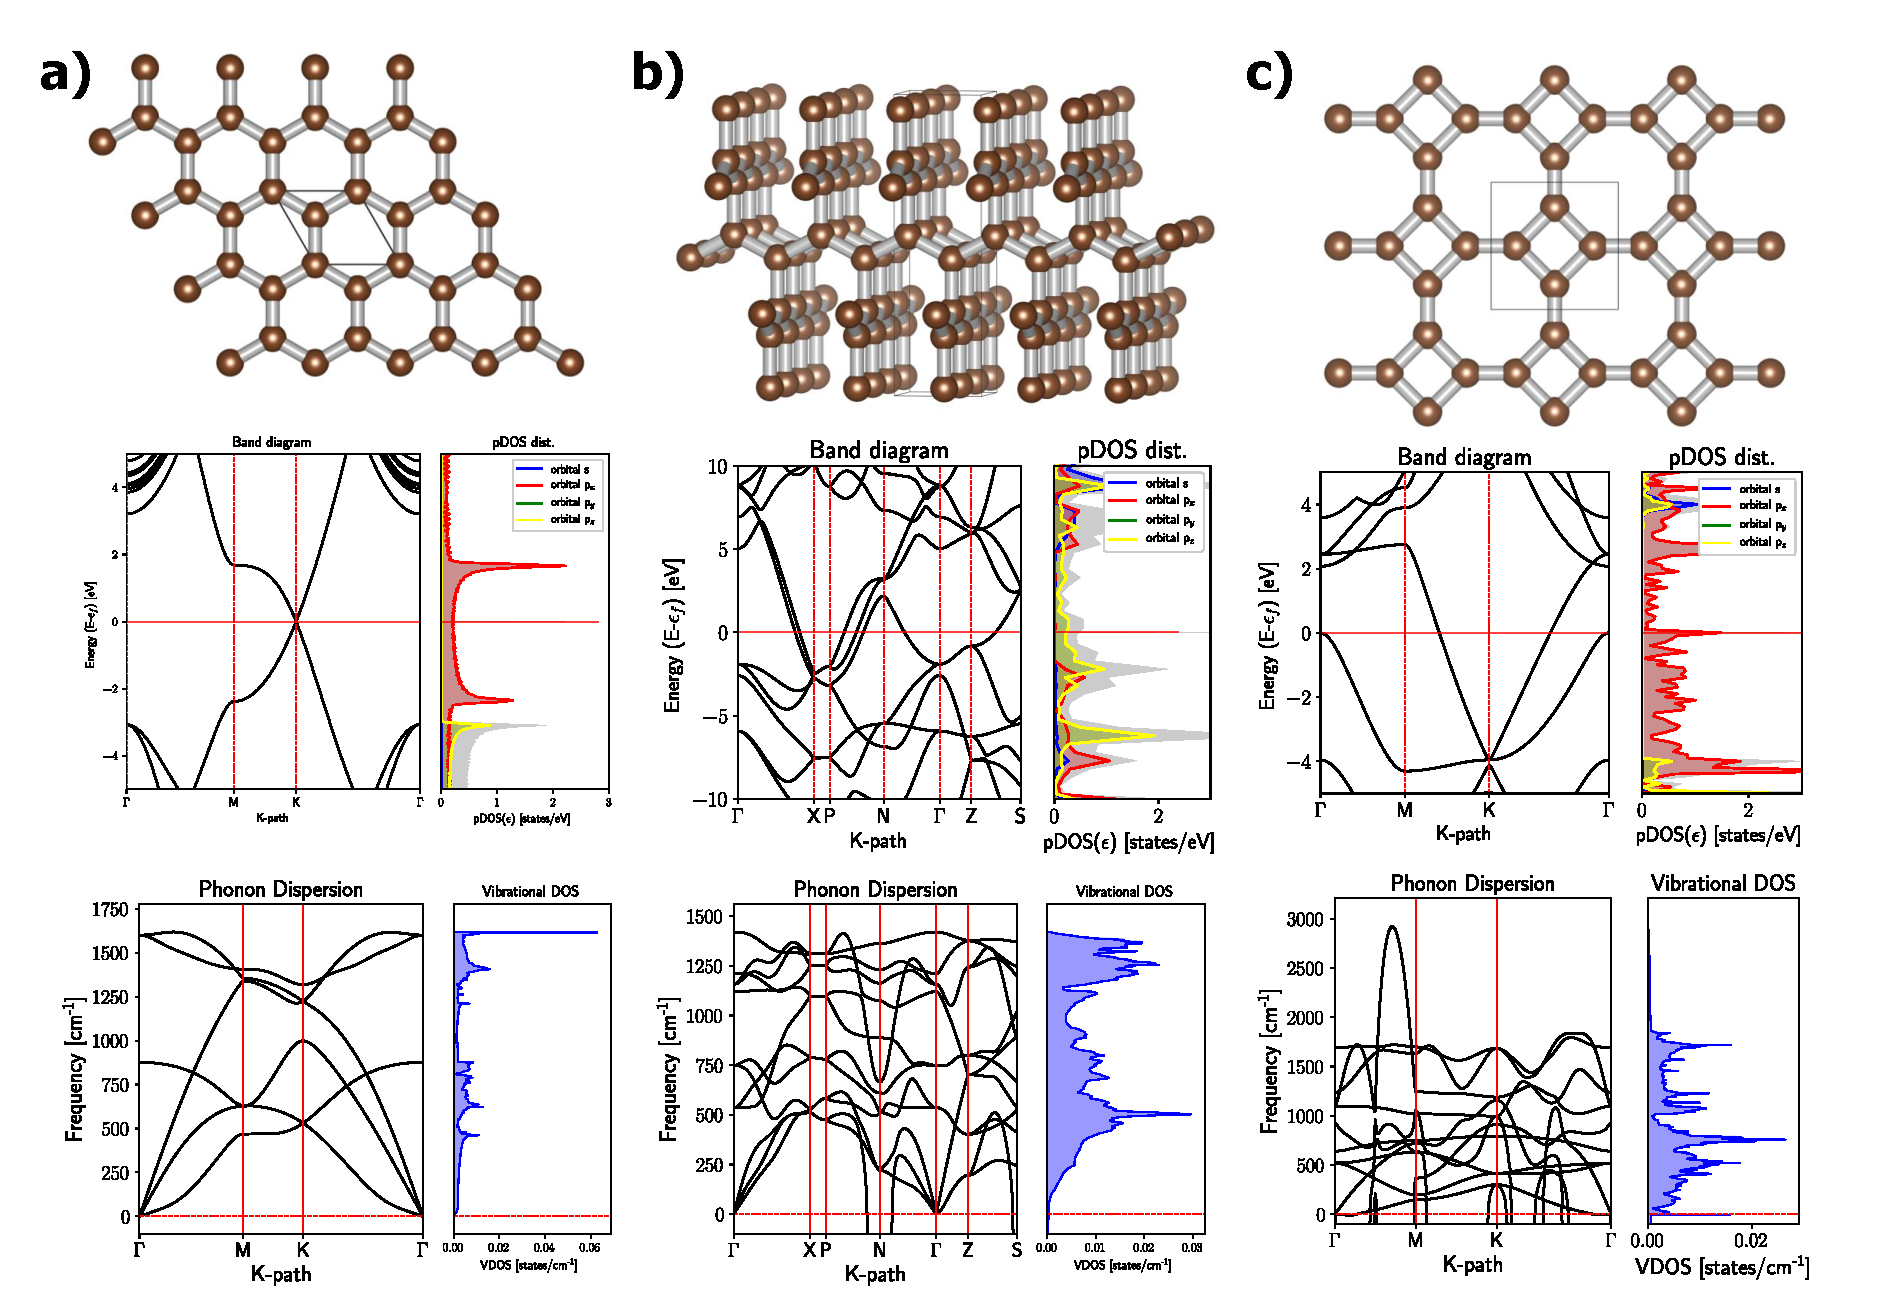
\includegraphics[width=1.\linewidth]{capitulos/fig/results3/0atoms}
			\caption{Diferentes alótropos que podem ser gerados a partir do carbino conectada diretamente.}
			\label{0atomos}
		\end{figure}
		
	\section{Conectando as cadeias por um átomo}
		
		Conectando as cadeias por um átomo pode-se gerar duas estruturas diferentes, sendo ambas tridimensionais. A primeira estrutura, derivada do carbino \textit{zigue-zague}, apresenta uma geometria parecida com a do bct-4, mas com as cadeias conectadas por duas ligações duplas cumulências (\autoref{1atomos}-\textbf{a}). A segunda é derivada do carbino \textit{armchair}, e já foi explorada na \autoref{sec:spiro} tendo sido denominada Spiro-Carbon (\autoref{1atomos}-\textbf{b}). Nenhuma das duas estruturas haviam sido relatadas na literatura anteriormente a esse trabalho. 
		
		\begin{figure}[!ht]
			\centering
			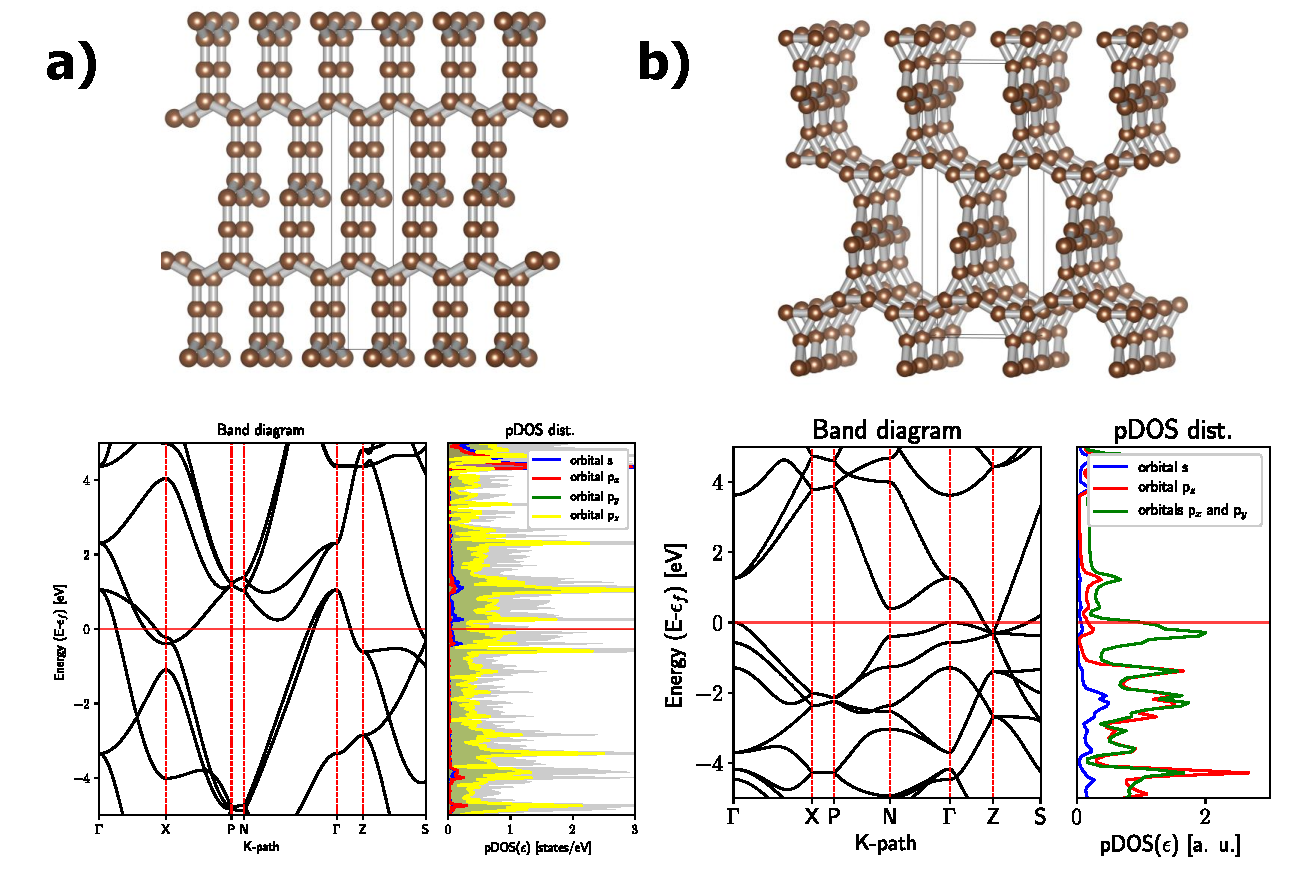
\includegraphics[width=1\linewidth]{capitulos/fig/results3/1atoms}
			\caption{Diferentes alótropos que podem ser gerados a partir do carbino conectada por um átomo de carbono.}
			\label{1atomos}
		\end{figure}
	
		Nenhuma das duas apresentaram frequências imaginárias na dispersão de fônons, indicando que as estruturas são um mínimo na superfície de energia potencial. Além disso, ambas as estruturas apresentam caráter eletrônico metálico com grande densidade de estados próximo ao nível de Fermi, uma consequência do caráter \textit{quasi}-unidimensional da cadeia do carbino.  
			
		
	\section{Conectando as cadeias por dois átomo ou mais átomos}
		
		Conectando as cadeias por dois átomos podemos gerar pelo menos quatro estruturas diferentes. Essa estratégia pode ser comparada a adicionar uma unidade acetilênica (-C$\equiv$C-) entre as cadeias do carbino distorcida, entretanto esses átomos têm a liberdade de apresentar ligações acetilênicas (ligando-se entre sí por ligações triplas e com seus vizinhos por ligações simples) ou ligações cumulênicas (formando uma sequência de três ligações duplas com orbitais $\pi$ perpendiculares). Das quatro estruturas possíveis, três são bidimensionais e somente uma tridimensional.   
		
		\begin{figure}[!ht]
			\centering
			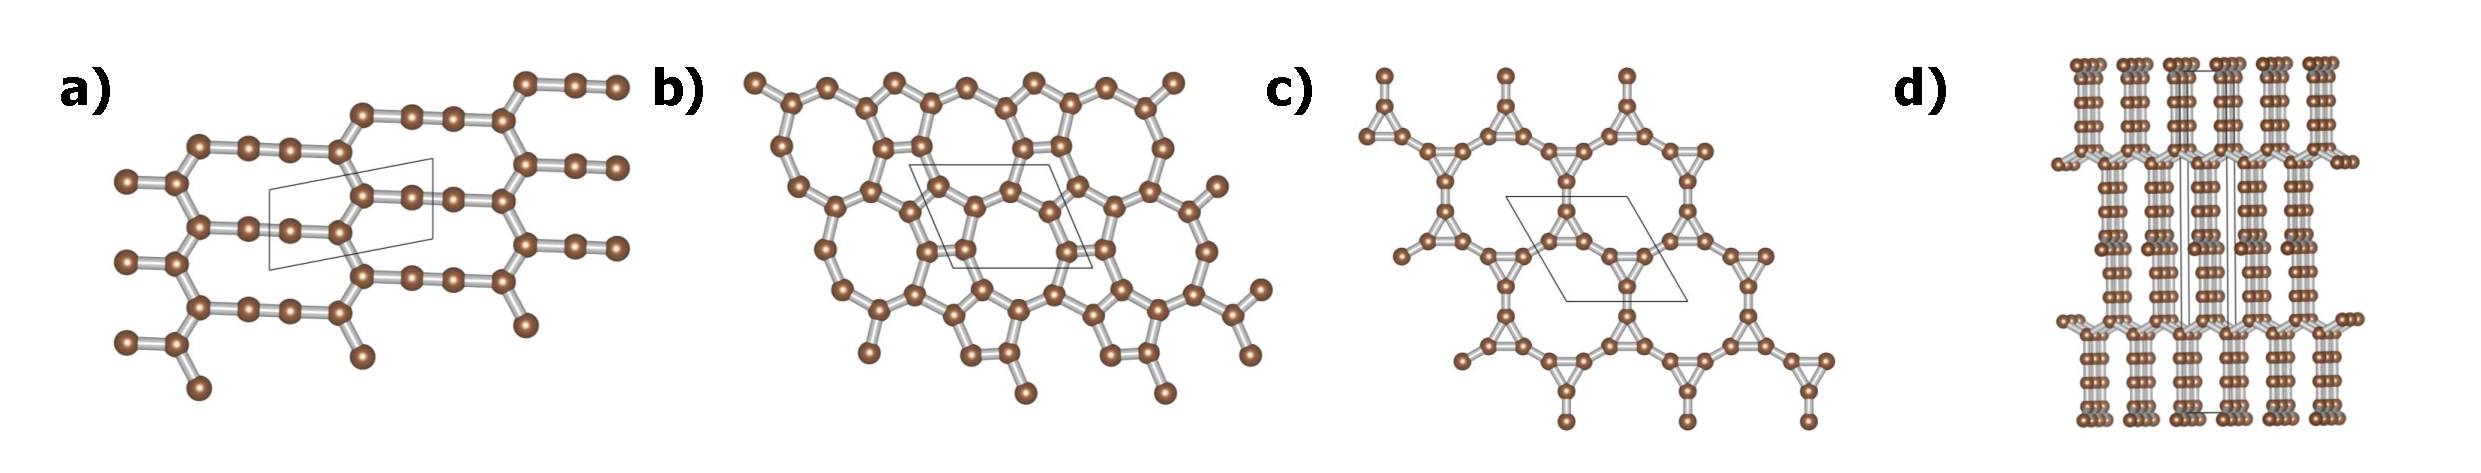
\includegraphics[width=1\linewidth]{capitulos/fig/results3/2atoms}
			\caption{Diferentes alótropos que podem ser gerados conectando cadeias do carbino por dois átomos de carbono.}
			\label{2atomos}
		\end{figure}	
		
		Ao tentar conectar as cadeias por três ou mais átomos, é possível notar que a estrutura geral passa a seguir o mesmo padrão, porém agora com mais átomos entre as cadeias principais. Por exemplo, ao conectar o carbino \textit{armchair} por três átomos o motivo estrutural semelhante ao \textit{Spiro-Carbon} aparece, mas agora os anéis de três membros estão separados por um átomo de carbono e não mais ligados diretamente. O mesmo acontece com as cadeias \textit{zigue-zague} conectadas por três átomos, estruturalmente ela fica muito parecida com a conectada por apenas um átomo porém agora as cadeias do carbino estão mais espaçadas. 
		
		Por fim é importante ressaltar que o conceito geral de gerar novos alótropos segundo as direções das distorções provenientes dos modos normais de vibração não está limitado ao carbino. Podemos pensar em estruturas 3D, como o diamante ou o Lonsdaleite, como sendo formado por distorções seguindo os modos normais de vibração do grafeno, por exemplo. Seguindo essa mesma lógica, outros materiais 2D podem ser distorcidos e conectados para gerar novas estruturas tridimensionais. Isso abre intrigantes e excitantes perspectivas para pesquisas futuras, mostrando como ainda somente arranhamos a superfície de todo o potencial estrutural que um único tipo de átomo pode gerar. 
	
		
	\section{Conclusões}
		
		Neste capítulo foi explorado o conceito de obtenção de novos alótropos a partir de um alótropo já conhecido, o carbino. Seguindo a distorção de cadeia na direção de um de seus modos normais de vibração e combinando as cadeias de maneira paralela ou perpendicular é possível obter a estrutura de alótropos já conhecidos como o grafeno e o bct-4 carbon. Adicionando um ou mais átomos entre as cadeias é possível conceber uma variedade de novas estruturas, com propriedades eletrônicas completamente diferentes. 
		
		Esse conceito abre espaço para novas pesquisas futuras, utilizando não somente o carbino como "bloco de construção" para novos alótropos, mas também outras estruturas como o grafeno e nanotubos de carbono. Essa estratégia permite a criação de um espaço amostral de possíveis estruturas de maneira simples e objetiva, facilitando a busca pelas estruturas mais estáveis e/ou que apresentem propriedades especiais, e assim incentivando esforços experimentais para sintetizar alguns candidatos. 